\documentclass[12pt, a4paper]{scrartcl}

\usepackage{ucs}
\usepackage[utf8x]{inputenc}
\usepackage[T1]{fontenc}
\usepackage{amsmath,amssymb,amstext}
\usepackage{graphicx}
\usepackage{textgreek}
\usepackage{framed,xcolor}
\usepackage[format=hang,indention=-1.2cm,font=footnotesize]{caption}
\usepackage{soul}
\setlength{\parindent}{0.5cm} 
\setlength{\parskip}{0.35cm}
\usepackage{setspace}
\usepackage{float}
\usepackage[numbib]{tocbibind}
\usepackage{sectsty}
\usepackage{enumitem}
\sectionfont{\Large}
\subsectionfont{\large}

\usepackage{geometry}
\geometry{a4paper, top=2.88cm, bottom=3.5cm, left=2.4cm, right=2.4cm}

\usepackage{enumitem}
\usepackage{hyperref}
\usepackage{courier}
\usepackage{listings}
\lstset{basicstyle=\small\ttfamily}

\author{David Kleindienst}
\title{Darea - Handbook}
\begin{document}
\maketitle
\section{Introduction}
Darea (\textbf{D}eep learning-\textbf{a}ssisted \textbf{re}plica image \textbf{a}nalysis suite) is a software designed for high-througput analysis of SDS-digest freeze-fracture replica immunogold electron microscopy images. It's features include: Automatic and manual demarcation of regions of interest, automatic and manual annotation of gold particles of different sizes, quantification of gold particle number and density and distances between gold particles as well as Monte-Carlo simulations of randomly distributed gold particles.

\tableofcontents
\section{Installation}
\subsection{Hardware Requirements}
Most functions of DareIt (including deep-learning prediction of demarcation) should run on any reasonably modern computer. The only exception to this is training neural network for demarcation prediction, for which we highly recommend using a modern NVIDIA GPU (at least 8GB memory). It will also run on CPU, but may take very long time (weeks) to finish.
\subsection{Software Prerequisites}
\begin{itemize}
\item Matlab R2018b or later with Simulink, Deep-learning toolbox and (optional but recommended) Parallel-processing toolbox
\item Python 3.6 (Anaconda distribution is highly recommended: \url{https://www.anaconda.com/distribution/})
\item For GPU: CUDA 9 (see \ref{cuda_ver} when wanting to use a different version)
\end{itemize}
\subsection{Installation}
The installation guide assumes that python was installed by Anaconda Distribution.
\subsubsection{Windows - CPU}
\textit{(tested on windows 7 and 10)}

In anaconda prompt run
\begin{lstlisting}[belowskip=0pt]
 conda env create -f <path to Darea>/envs/Darea_Windows.yml
\end{lstlisting}
It is now downloading and installing neccessary packages which may take some time. After it finished, run
\begin{lstlisting}[belowskip=0pt]
 conda activate Darea
 where python
\end{lstlisting}
the last command will give you a path:
now in matlab run: 
\begin{lstlisting}[belowskip=0pt]
 pyversion <path> 
\end{lstlisting}

(replace <path> with the output you got from where python command)
\subsubsection{Windows - GPU}
\textit{(tested on windows 7)}

In anaconda prompt run
\begin{lstlisting}[belowskip=0pt]
 conda env create -f <path to Darea>/envs/Darea_WindowsGPU.yml
\end{lstlisting}
It is now downloading and installing neccessary packages which may take some time. After it finished, run
\begin{lstlisting}[belowskip=0pt]
 conda activate Darea
 where python
\end{lstlisting}
the last command will give you a path:
now in matlab run: 
\begin{lstlisting}[belowskip=0pt]
 pyversion <path> 
\end{lstlisting}
(replace <path> with the output you got from where python command).
Please refer to \ref{cuda_ver} to ensure your CUDA and cudatoolkit versions match.

\subsubsection{MacOS - CPU}
\textit{(tested on MacOS Mojave)}

In terminal run
\begin{lstlisting}[belowskip=0pt]
 conda env create -f <path to Darea>/envs/Darea_MacOS.yml
\end{lstlisting}
It is now downloading and installing neccessary packages which may take some time. After it finished, run
\begin{lstlisting}[belowskip=0pt]
 conda activate Darea
 which python
\end{lstlisting}
the last command will give you a path:
now in matlab run: 
\begin{lstlisting}[belowskip=0pt]
 pyversion <path> 
\end{lstlisting}
(replace <path> with the output you got from where python command)
\subsubsection{MacOS - GPU}
\textit{(not tested)}

Follow the instructions for MacOS - CPU. Testing if it works is recommended at this step. Then, type in terminal:
\begin{lstlisting}[belowskip=0pt]
 conda activate Darea
 conda uninstall tensorflow tensorflow-base
 conda install tensorflow-GPU=1.12
\end{lstlisting}
Then follow \ref{cuda_ver} to make sure your CUDA and cudatoolkit versions match.
\subsubsection{Other operating systems or using other package managers than Anaconda}
Unfortunately, due to interplay between Matlab and python, this software is very sensitive to changes in package versions and it is a bit of a gamble if a version change in any of the packages will break the functionality. We recommend having a look at the package version information in any (or all) of the .yml files and trying to install a similar environment.
First get it running with CPU, then (if wanted) try to follow the MacOS-GPU guide to get it running on GPU.
\subsubsection{Using other versions of CUDA}
\label{cuda_ver}
in terminal run: 
\begin{lstlisting}[belowskip=0pt]
 nvcc --version 
\end{lstlisting}
to get the version number of CUDA
then (after installation) in anaconda prompt:
\begin{lstlisting}[belowskip=0pt]
 conda install cudatoolkit=<version>
\end{lstlisting}
Replace <version> by major version number returned by nvcc command, e.g. when using CUDA 10, run:
\begin{lstlisting}[belowskip=0pt]
 conda install cudatoolkit=10 
\end{lstlisting}
\section{Typical Workflow}
In a typical analysis workflow, first a project is created and images are imported (see \ref{m:create}). Typically labelings for different proteins are imported into different projects, while different experimental conditions (genotypes, brain regions, ...) are pooled into the same project. If images are provided as 8-bit, they should then be converted to 16-bit (see Fig. \ref{fig:MM} (6) ).
Images are then assigned into different groups (genotypes, brain regions, ...) (see \ref{m:groups}) and general project settings (e.g. which particle sizes, whether particles should be detected on ROI only) are set (see \ref{m:settings}). 
Automated demarcation and particle detection can then be run (see \ref{m:auto}). Resulting demarcations can then be revised manually (or performed manually if no automated demarcation was run) (see \ref{m:demarcate}) followed by manual revision of particle annotations (see \ref{m:particles}). 
After finishing annotation of the data, analysis and Monte-Carlo simulations should be run (see \ref{m:analysis}). From the results, data sheets and figures can be exported (see \ref{m:figures}) and example images can be created (see \ref{m:visualize}).
Annotated data can then be used to further refine automated demarcation (see \ref{m:trainDem}) and particle prediction (see \ref{m:trainPart}).

\section{The Main Menu}
To run Darea, start MATLAB. Navigate to the Darea folder and you should see a file named "run.m". Right click on the file and select run from the menu. Now Darea's main menu (Fig. \ref{fig:MM}) should open.

\begin{figure}[H]
\includegraphics[width=\linewidth]{screenshots/scr_mainmenu.png}
\captionsetup{singlelinecheck=off}
\caption[thing]{Darea Main Menu
\begin{enumerate}[label=\textbf{\arabic*:}, leftmargin=1.88\parindent]
\item Create a new project and import images (see \ref{m:create})
\item Load existing project
\item Shows the path to the currently loaded project file
\item Add and remove images and modify scale (see \ref{m:manage})
\item Set, for example, which particle sizes exist and how far from the demarcation they should be detected (see \ref{m:settings})
\item Assign groups to images (see \ref{m:groups})
\item Preprocessing of images. Includes converting images to 16 bit, autoadjusting contrast and inverting the images. See \ref{m:preprocess} for details. \textbf{Warning: This modifies the original image files!}
\item Manual image demarcation (see \ref{m:demarcate})
\item Manual gold particle annotation (see \ref{m:particles})
\item Run analysis and (if desired) Monte-Carlo simulations (see \ref{m:analysis})
\item Generate data tables and figures (see \ref{m:figures})
\item Visualize the results and generate publication ready example images (see \ref{m:visualize})
\item Automatically annotate demarcation and gold particles (see \ref{m:auto})
\item Train machine learning algorithm for automated gold particle annotation (see \ref{m:trainPart})
\item Train neural network for automated demarcation (see \ref{m:trainDem})
\end{enumerate}}
\label{fig:MM}
\end{figure}

\section{Projects and Groups}
\subsection{Creating projects and importing images}
\subsubsection{Image requirements and suggested folder structure}
\label{folderstruct}
Images have to be provided as 8 or 16 bit rgb or grayscale .tif images. When images of different magnifications are used, we recommend saving the magnification (separated by some deliminator) to the filename, as this allows automatic detection of the appropriate scale. Where in the filename the magnification occurs is irrelevant. Examples of usable filenames (we here use 39000x as example magnification, but it can really be anything and does not have to contain an x): 01\_39000x.tif ; Hippocampus\_39000x\_image1.tif ; 39000x\_01.tif ; 01-39000x.tif ; 39000x\#image1.tif. Examples of filenames where the magnification would not be detected correctly (because the deliminator is lacking): Image39000x.tif ; 39000xImage.tif

For optimal automatic importing of your images we suggest the following structure:
\begin{figure}[H]
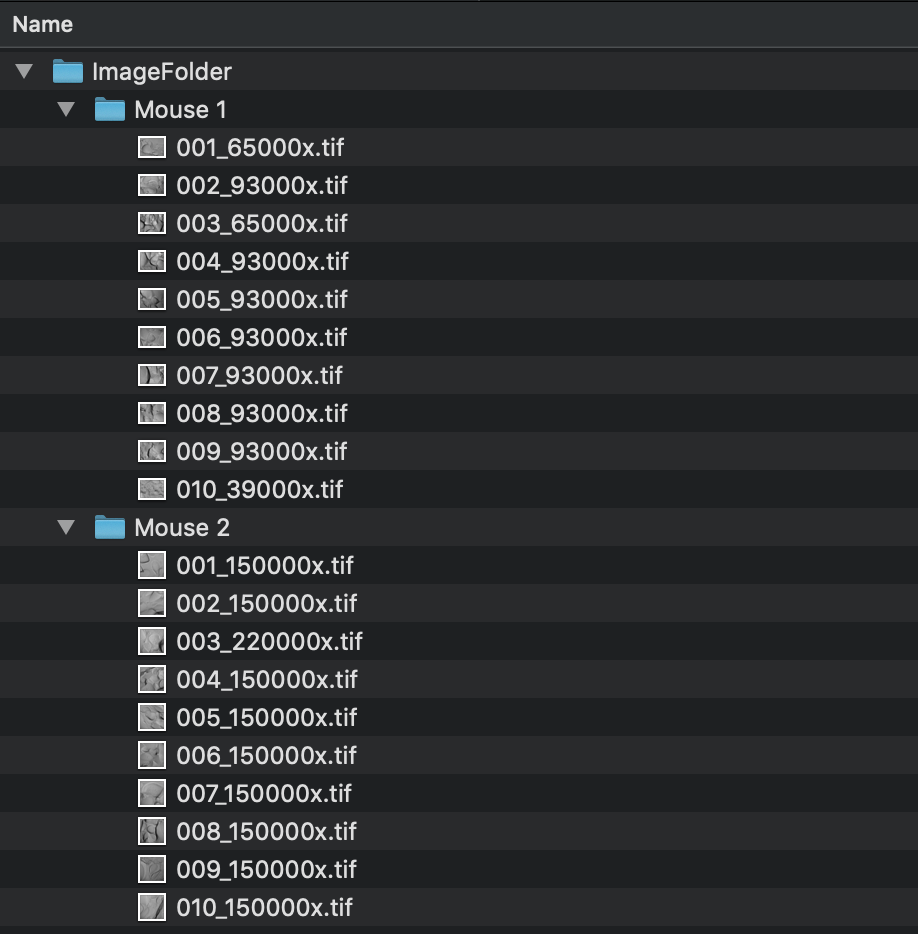
\includegraphics[scale=0.6]{screenshots/scr_folderstructure.png}
\captionsetup{singlelinecheck=off}
\caption[thing]{Suggested Folder structure.}
\end{figure}
In this case "ImageFolder" should be specified for importing, and during auto import the images will be assigned into the groups "Mouse 1" and "Mouse 2". This group assignment can be changed later (see \ref{m:groups}.
\subsubsection{Creating Projects}
\label{m:create}
\begin{figure}[H]
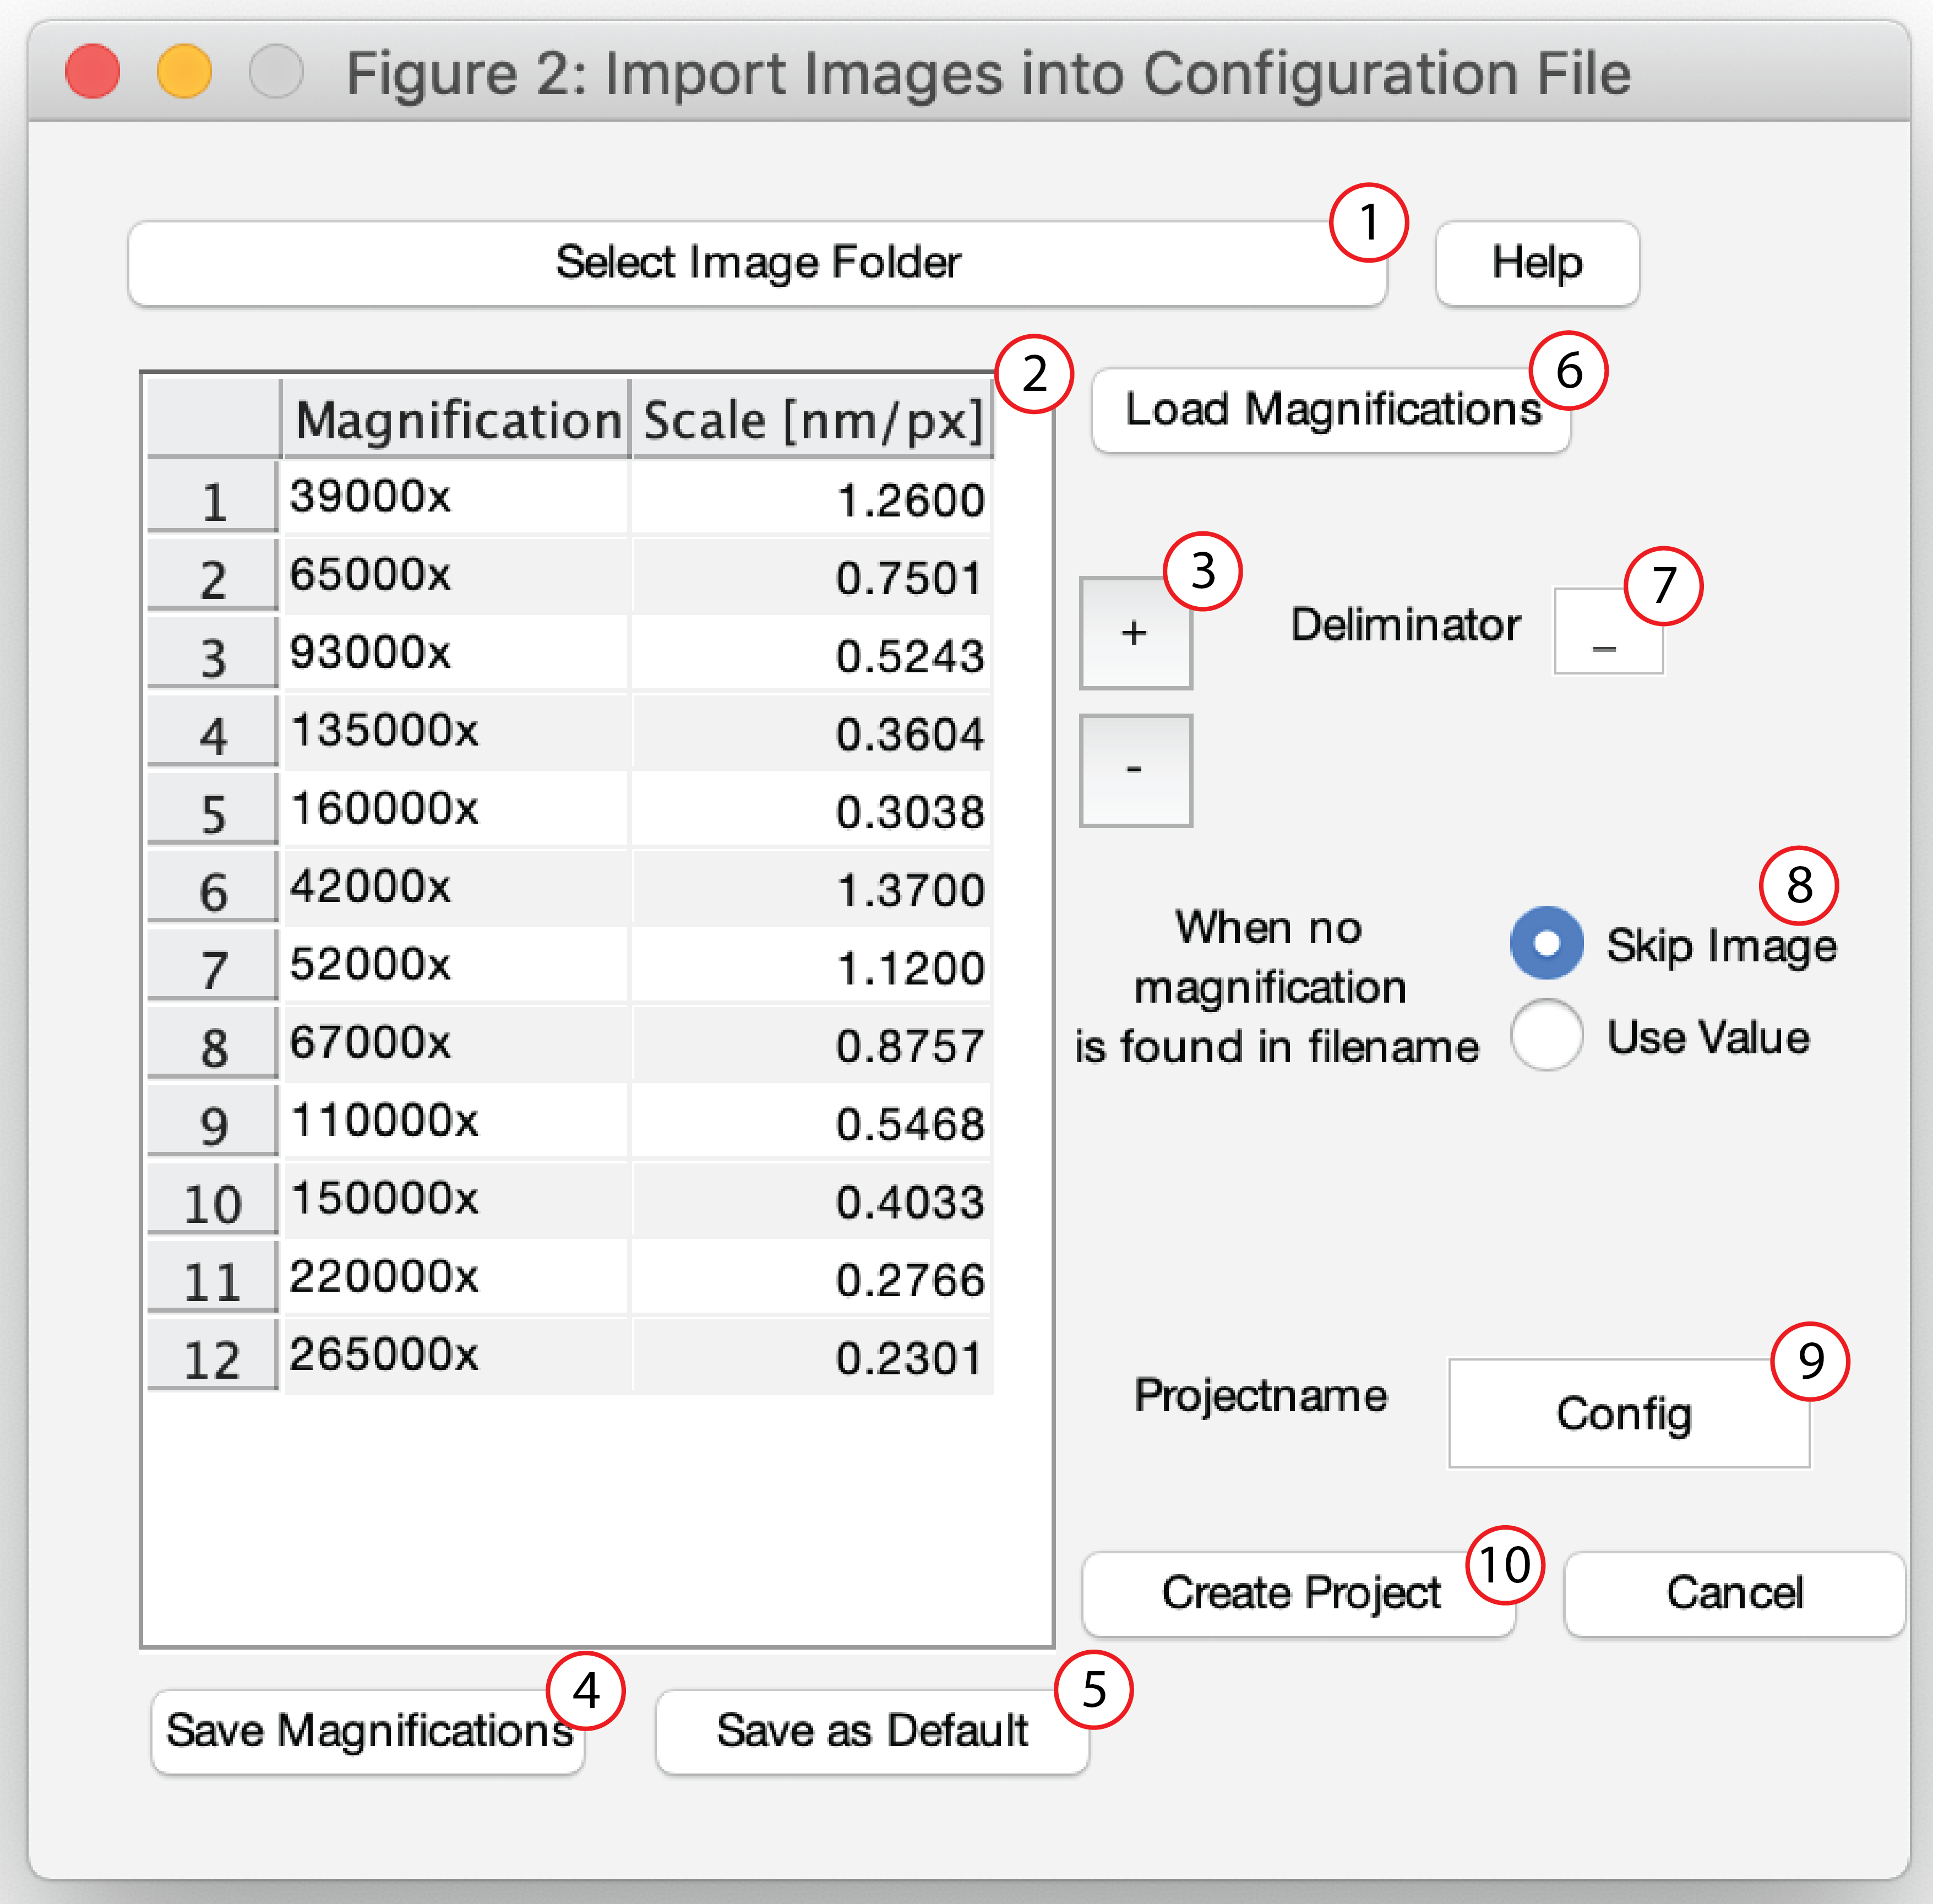
\includegraphics[scale=0.7]{screenshots/scr_CreateProject.png}
\captionsetup{singlelinecheck=off}
\caption[thing]{Create Project
\begin{enumerate}[label=\textbf{\arabic*:}, leftmargin=1.88\parindent]
\item Select the folder containing your image folders (see \ref{folderstruct}).
\item List of magnifications which should be detected in the filename. The left column indicates how the magnification is described in the filename, while the right column indicates the scale (in nm/px). In the displayed case an image called 01\_39000x.tif would be assigned a scale of 1.26 nm/px. 
\item Add another line to magnification list (+) or remove the currently selected line (-)
\item Save magnification list into a file
\item Save magnification list as future default which will be loaded automatically
\item Load magnification file 
\item The delimiter between magnfication and the rest of the filename. If your filename is 01\_39000x delimiter should be \_ ; if your filename is 01-39000x delimiter should be - .
\item Images that do not contain a valid magnfication (listed in 2) can be either ignored ("skip image") or assigned a specific scale ("use value" and specify the scale in the field that appears). The latter one is especially useful if all your images are the same magnfication and do not contain the magnification in the filename.
\item The name of this project. The project will than be saved in the image folder as \textit{projectname}.dat
\item Create the project
\end{enumerate}}
\end{figure}
\subsubsection{Managing Images}
\label{m:manage}
\begin{figure}[H]
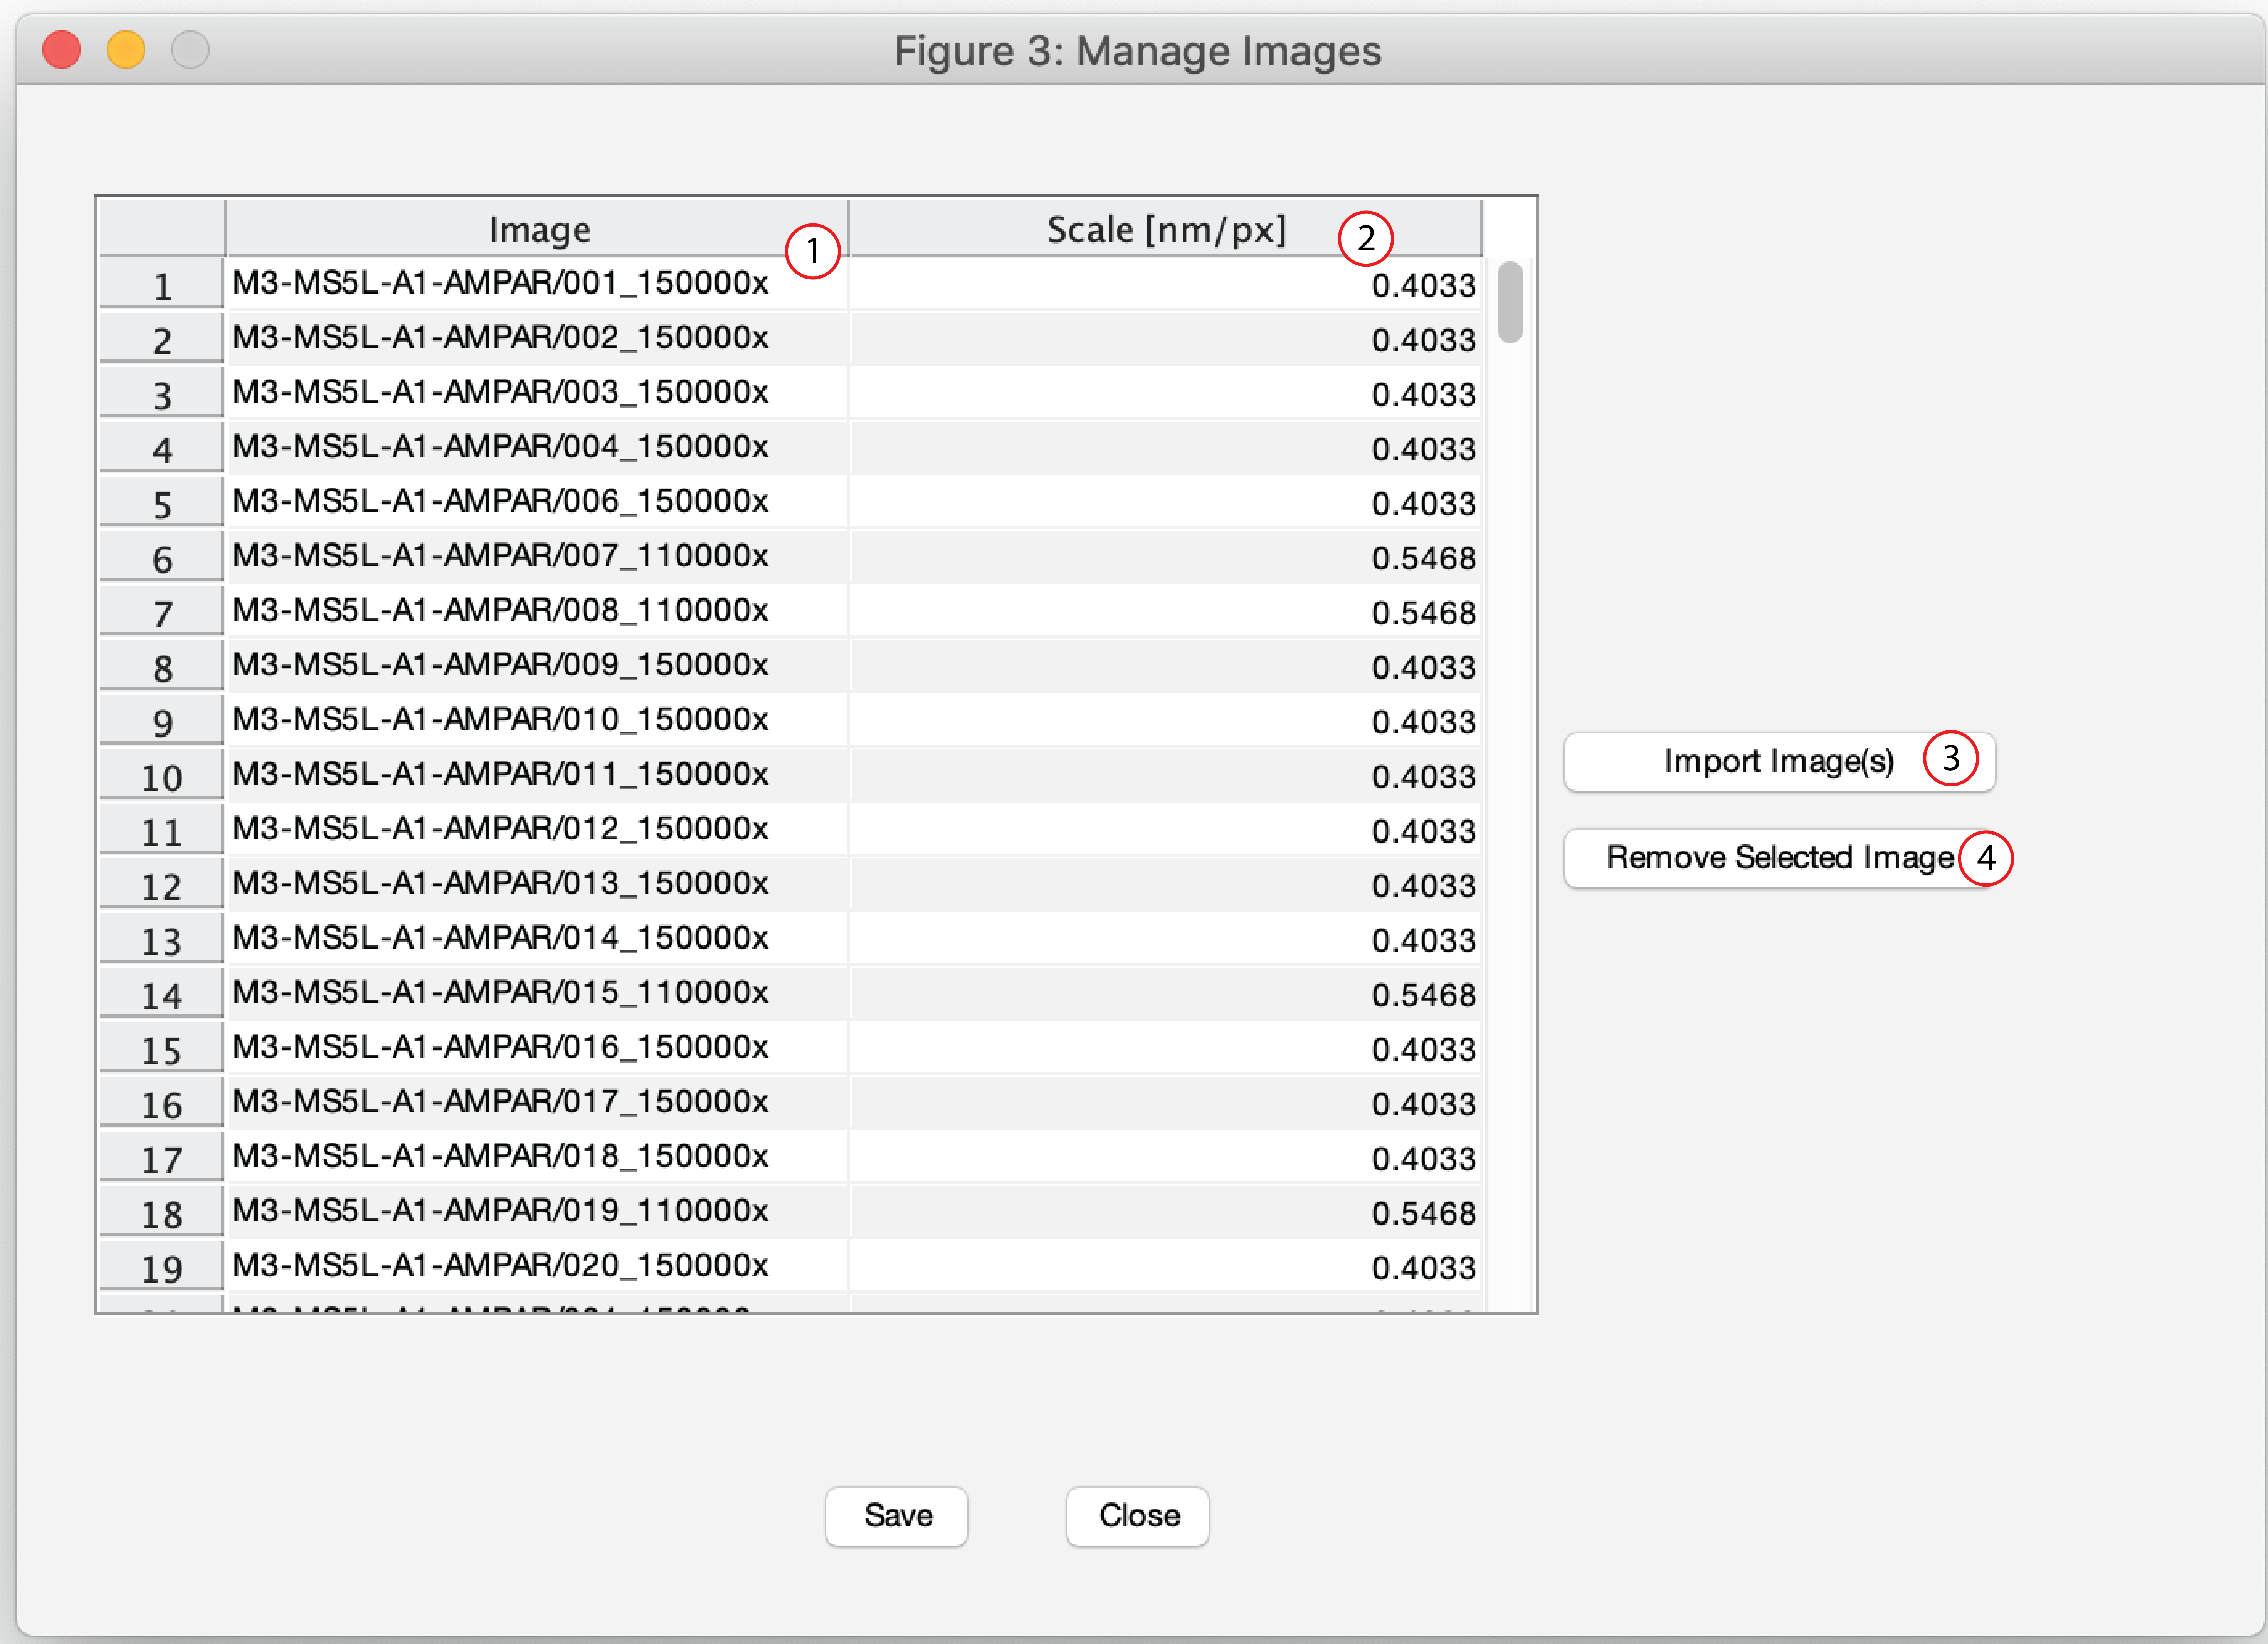
\includegraphics[scale=0.5]{screenshots/scr_Manage.png}
\captionsetup{singlelinecheck=off}
\caption[thing]{Manage Images
\begin{enumerate}[label=\textbf{\arabic*:}, leftmargin=1.88\parindent]
\item List of all the images
\item Scale for each image, click to modify.
\item Select one or multiple images to import into this project. They will then be added to the end of the list
\item Remove the selected image from the project
\end{enumerate}}
\end{figure}

\subsection{Project settings}
\label{m:settings}
\begin{figure}[H]
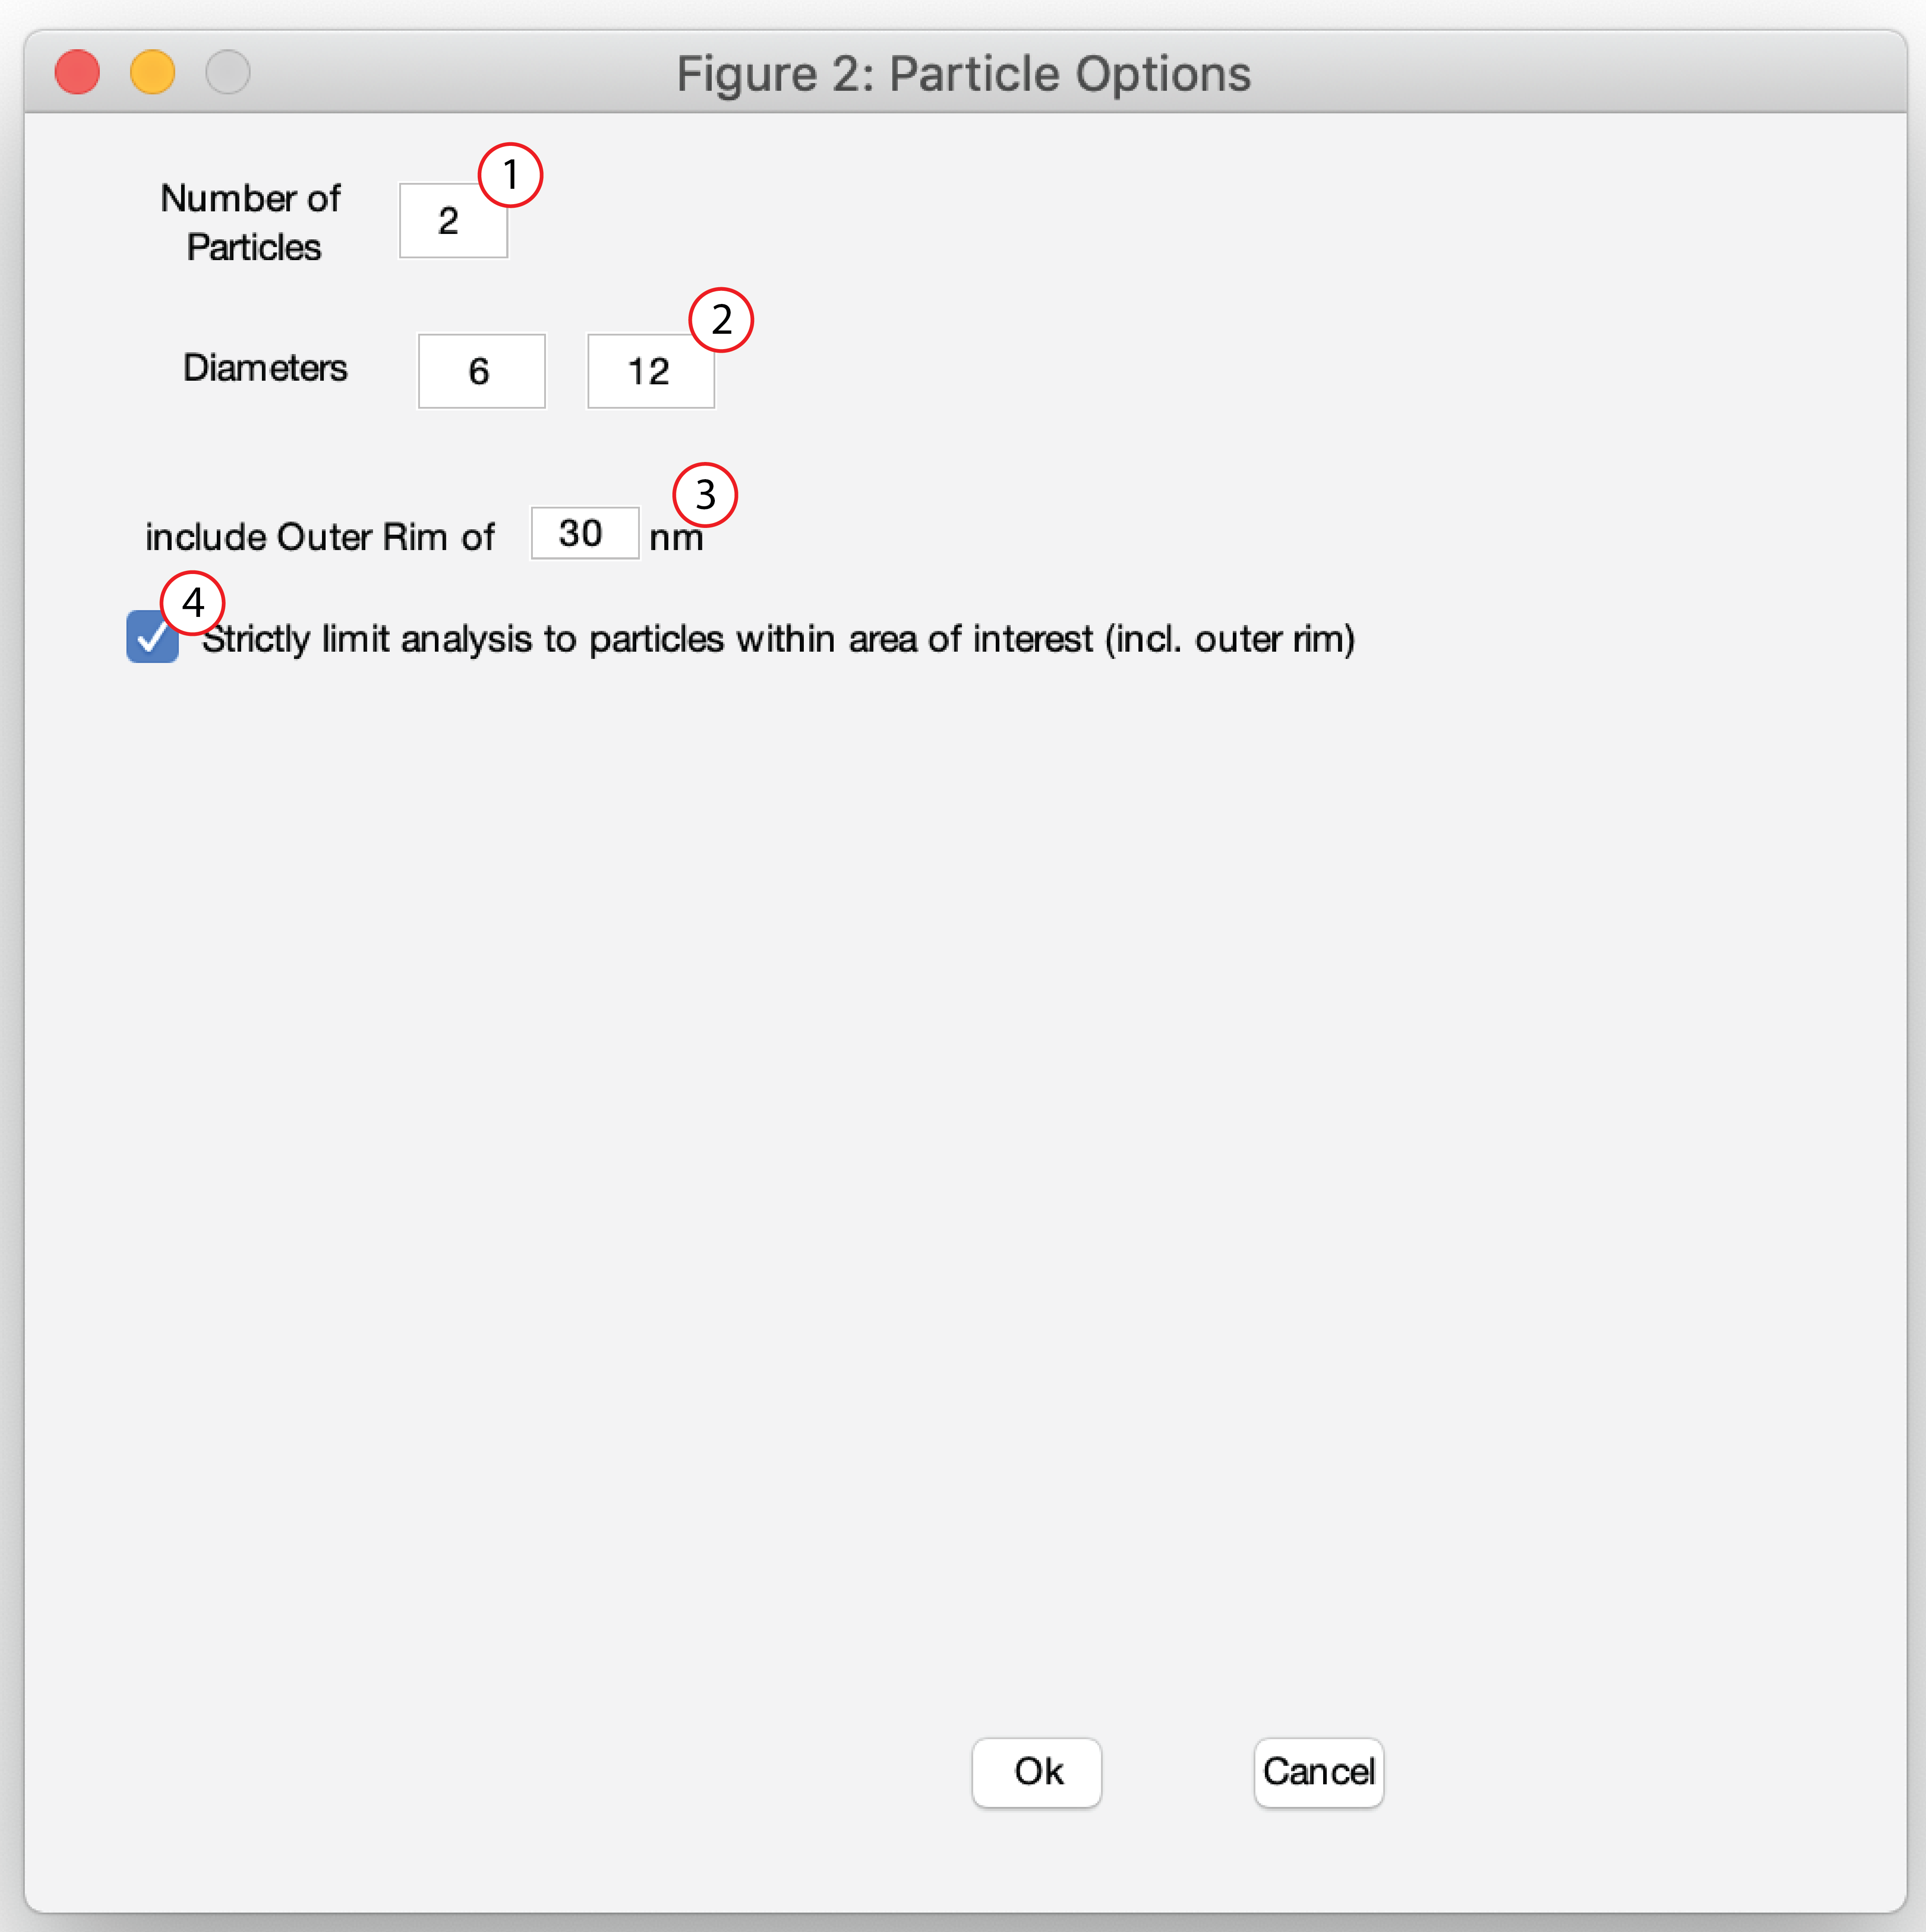
\includegraphics[scale=0.6]{screenshots/scr_Settings.png}
\captionsetup{singlelinecheck=off}
\caption[thing]{Project settings
\begin{enumerate}[label=\textbf{\arabic*:}, leftmargin=1.88\parindent]
\item How many different particle sizes you used
\item The different particle diameters (in nm)
\item Size of the outer rim around the demarcation within which particles should be detected.
\item If ticked, particles outside of both demarcation and outer rim will be ignored (usually that is the expected behavior)
\end{enumerate}}
\end{figure}
\subsection{Groups}
\label{m:groups}
Groups can be specified at any time before figures and tables are made.
\begin{figure}[H]
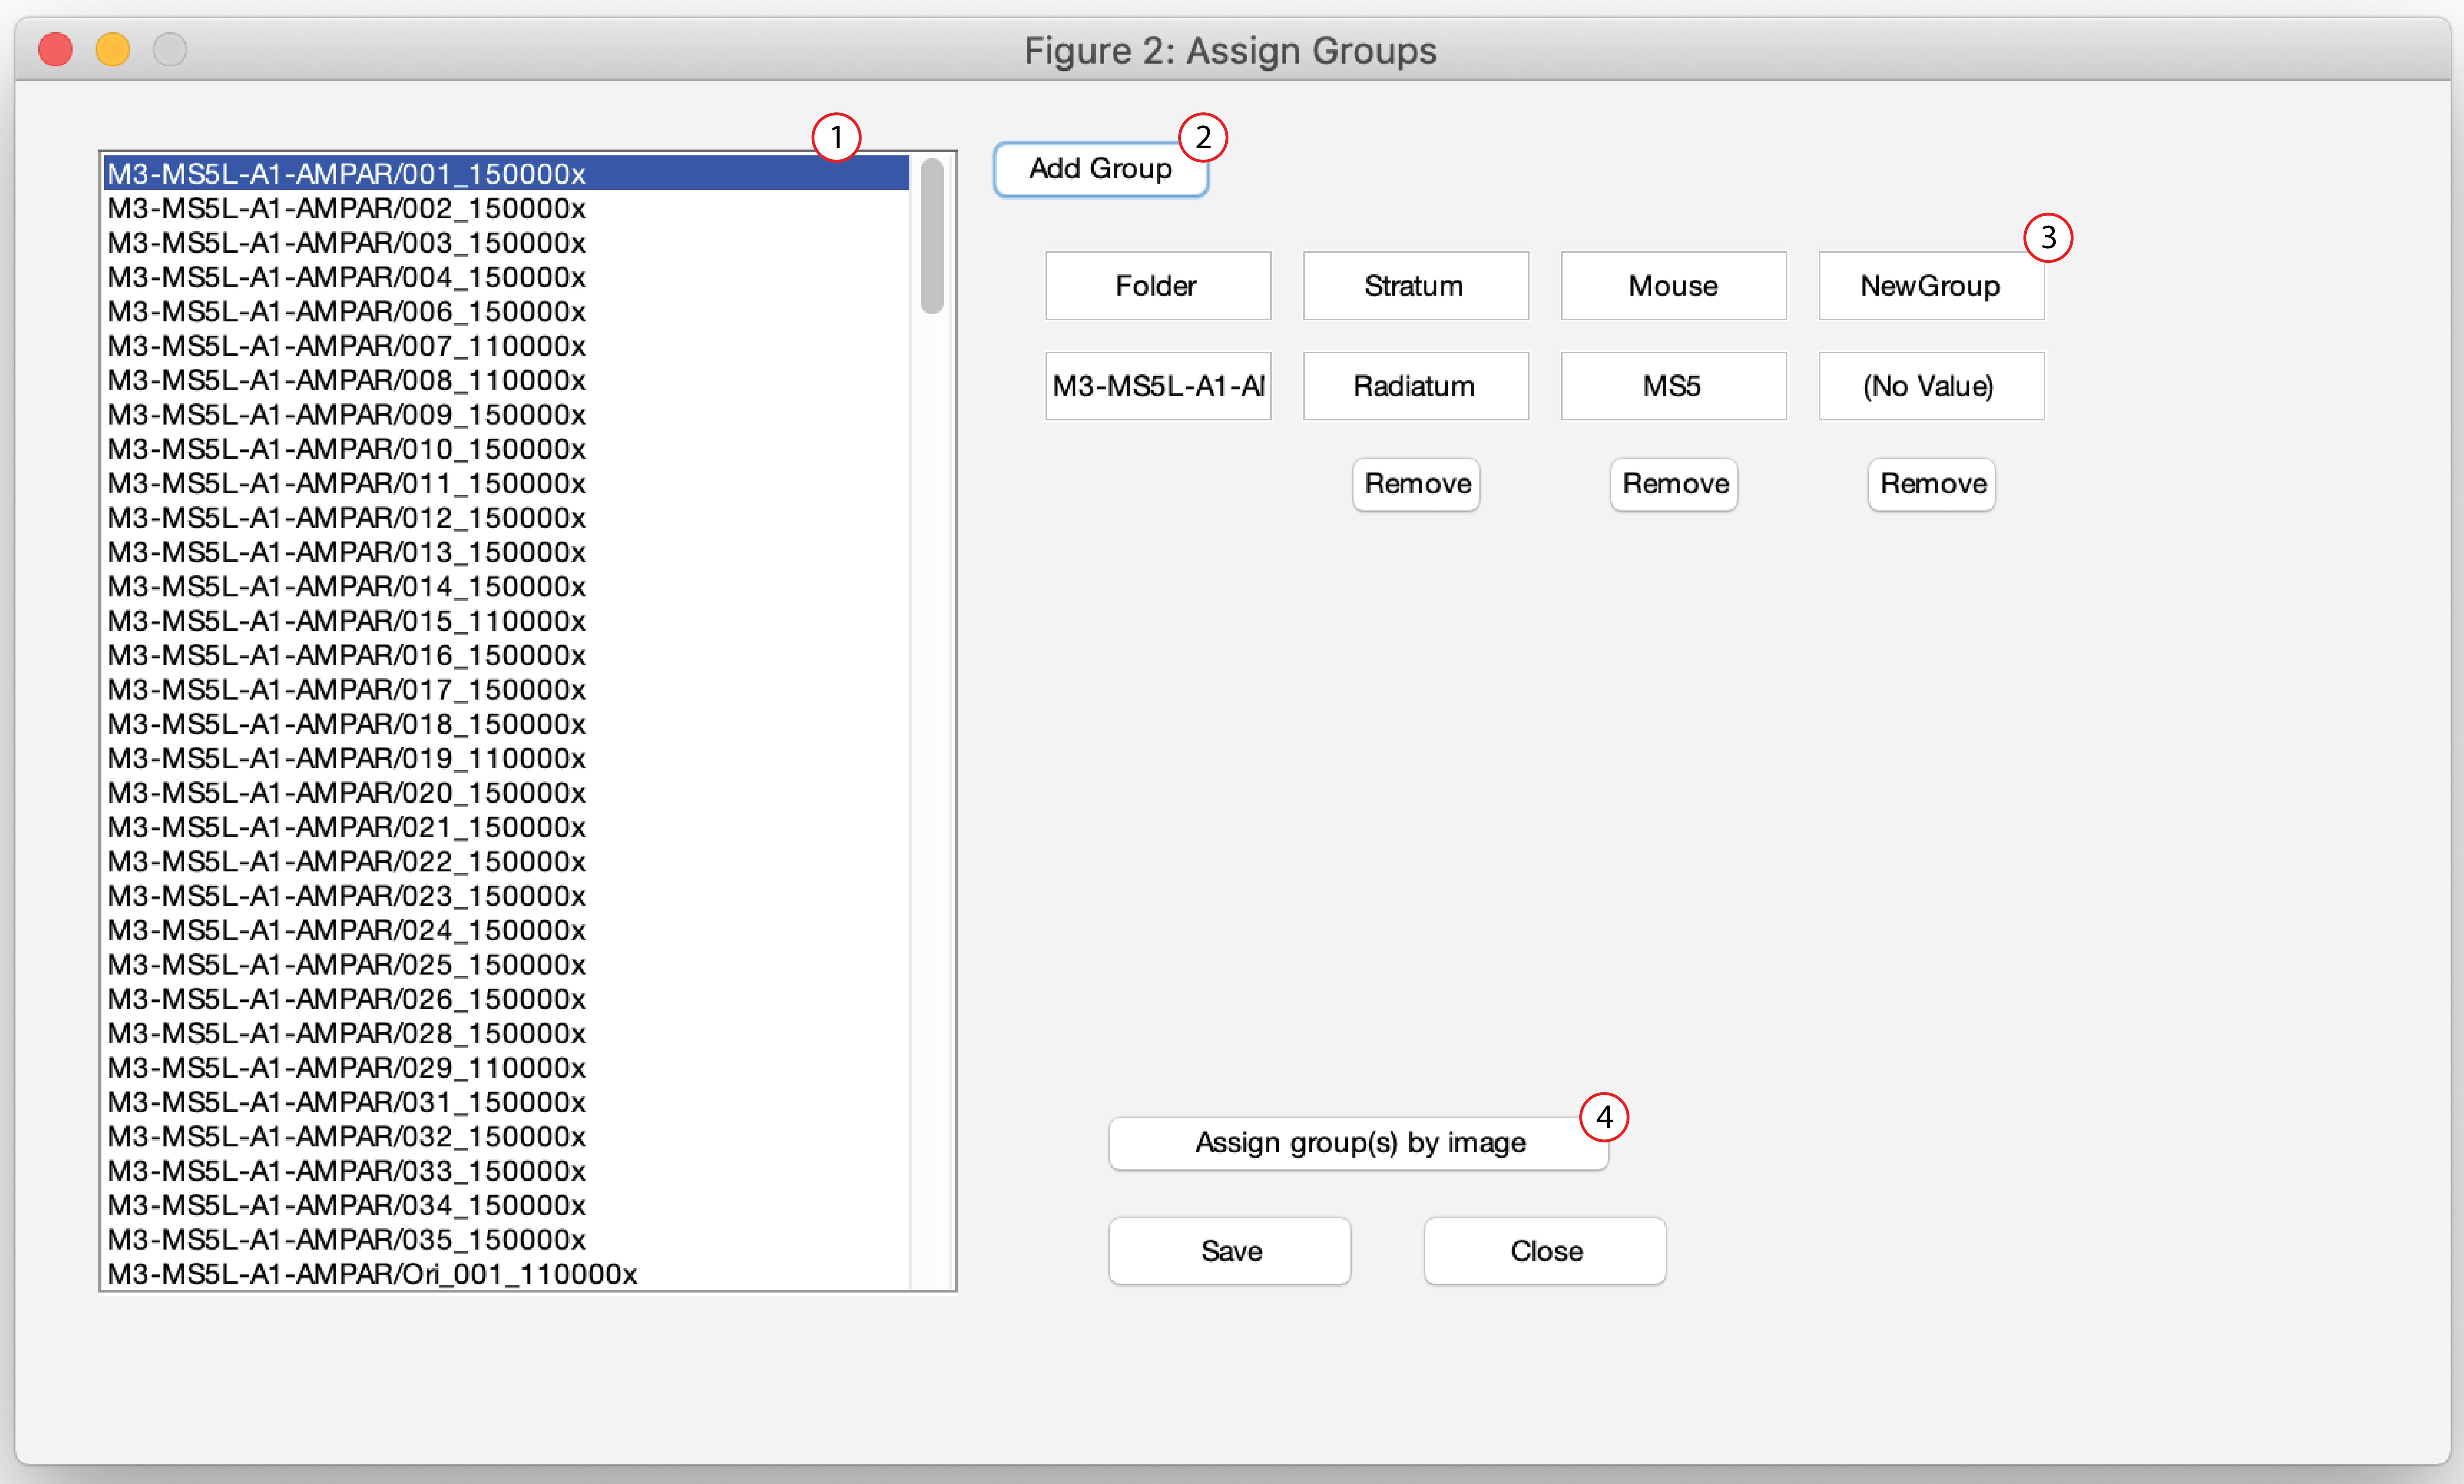
\includegraphics[width=\linewidth]{screenshots/scr_Groups.png}
\captionsetup{singlelinecheck=off}
\caption[thing]{Groups
\begin{enumerate}[label=\textbf{\arabic*:}, leftmargin=1.88\parindent]
\item List of all images. Multiple images can be selected using shift or ctrl.
\item Add a new grouping, i.e. a property by which images can be divided into different groups (e.g. brain region, genotype, animal number).
\item Each column contains a grouping. The top row has the names of the groupings (e.g. brain region, genotype), these are the same for all images. The bottom row has the individual groupnames (e.g. hippocampus, wild-type) which may differ between images. Modifying this value will change it for all images selected in (1).
\item Sometimes, you may want to assign groups based on a property of the image (e.g. complete and incomplete profiles or perforated and non-perforated synapses). Assign group by image will show you each image and let you assign a group individually (see \ref{m:grpbyimg}).
\end{enumerate}}
\end{figure}
\subsubsection{Assign group by image}
\label{m:grpbyimg}
\begin{figure}[H]
\includegraphics[scale=0.66]{screenshots/scr_assign_1.png}
\captionsetup{singlelinecheck=off}
\caption[thing]{Assign groups by image
\begin{enumerate}[label=\textbf{\arabic*:}, leftmargin=1.88\parindent]
\item Select which grouping(s) should be assigned for each image
\item Whether or not the demarcation (if it exists) should be indicated
\end{enumerate}}
\end{figure}

\begin{figure}[H]
\includegraphics[scale=0.66]{screenshots/scr_assign_2.png}
\captionsetup{singlelinecheck=off}
\caption[thing]{Assign groups by image
\begin{enumerate}[label=\textbf{\arabic*:}, leftmargin=1.88\parindent]
\item Specify which are the possible groups, separated by ";"s.  In this example each image will be assigned to Group A, B or C.
\end{enumerate}}
\end{figure}
\begin{figure}[H]
\includegraphics[width=\linewidth]{screenshots/scr_assign_3.png}
\captionsetup{singlelinecheck=off}
\caption[thing]{Assign groups by image
\begin{enumerate}[label=\textbf{\arabic*:}, leftmargin=1.88\parindent]
\item Click the corresponding button (or hotkey, shown between []) to assign a group to the image. Once you assign a group, the next image will be opened. This will continue until all images were assigned a group. If you cancel before going through all images, your inputs will not be saved!
\item Click back to go to the previous image to correct your choice. 
\end{enumerate}}
\end{figure}
\subsection{Preprocessing}
\label{m:preprocess}
\begin{figure}[H]
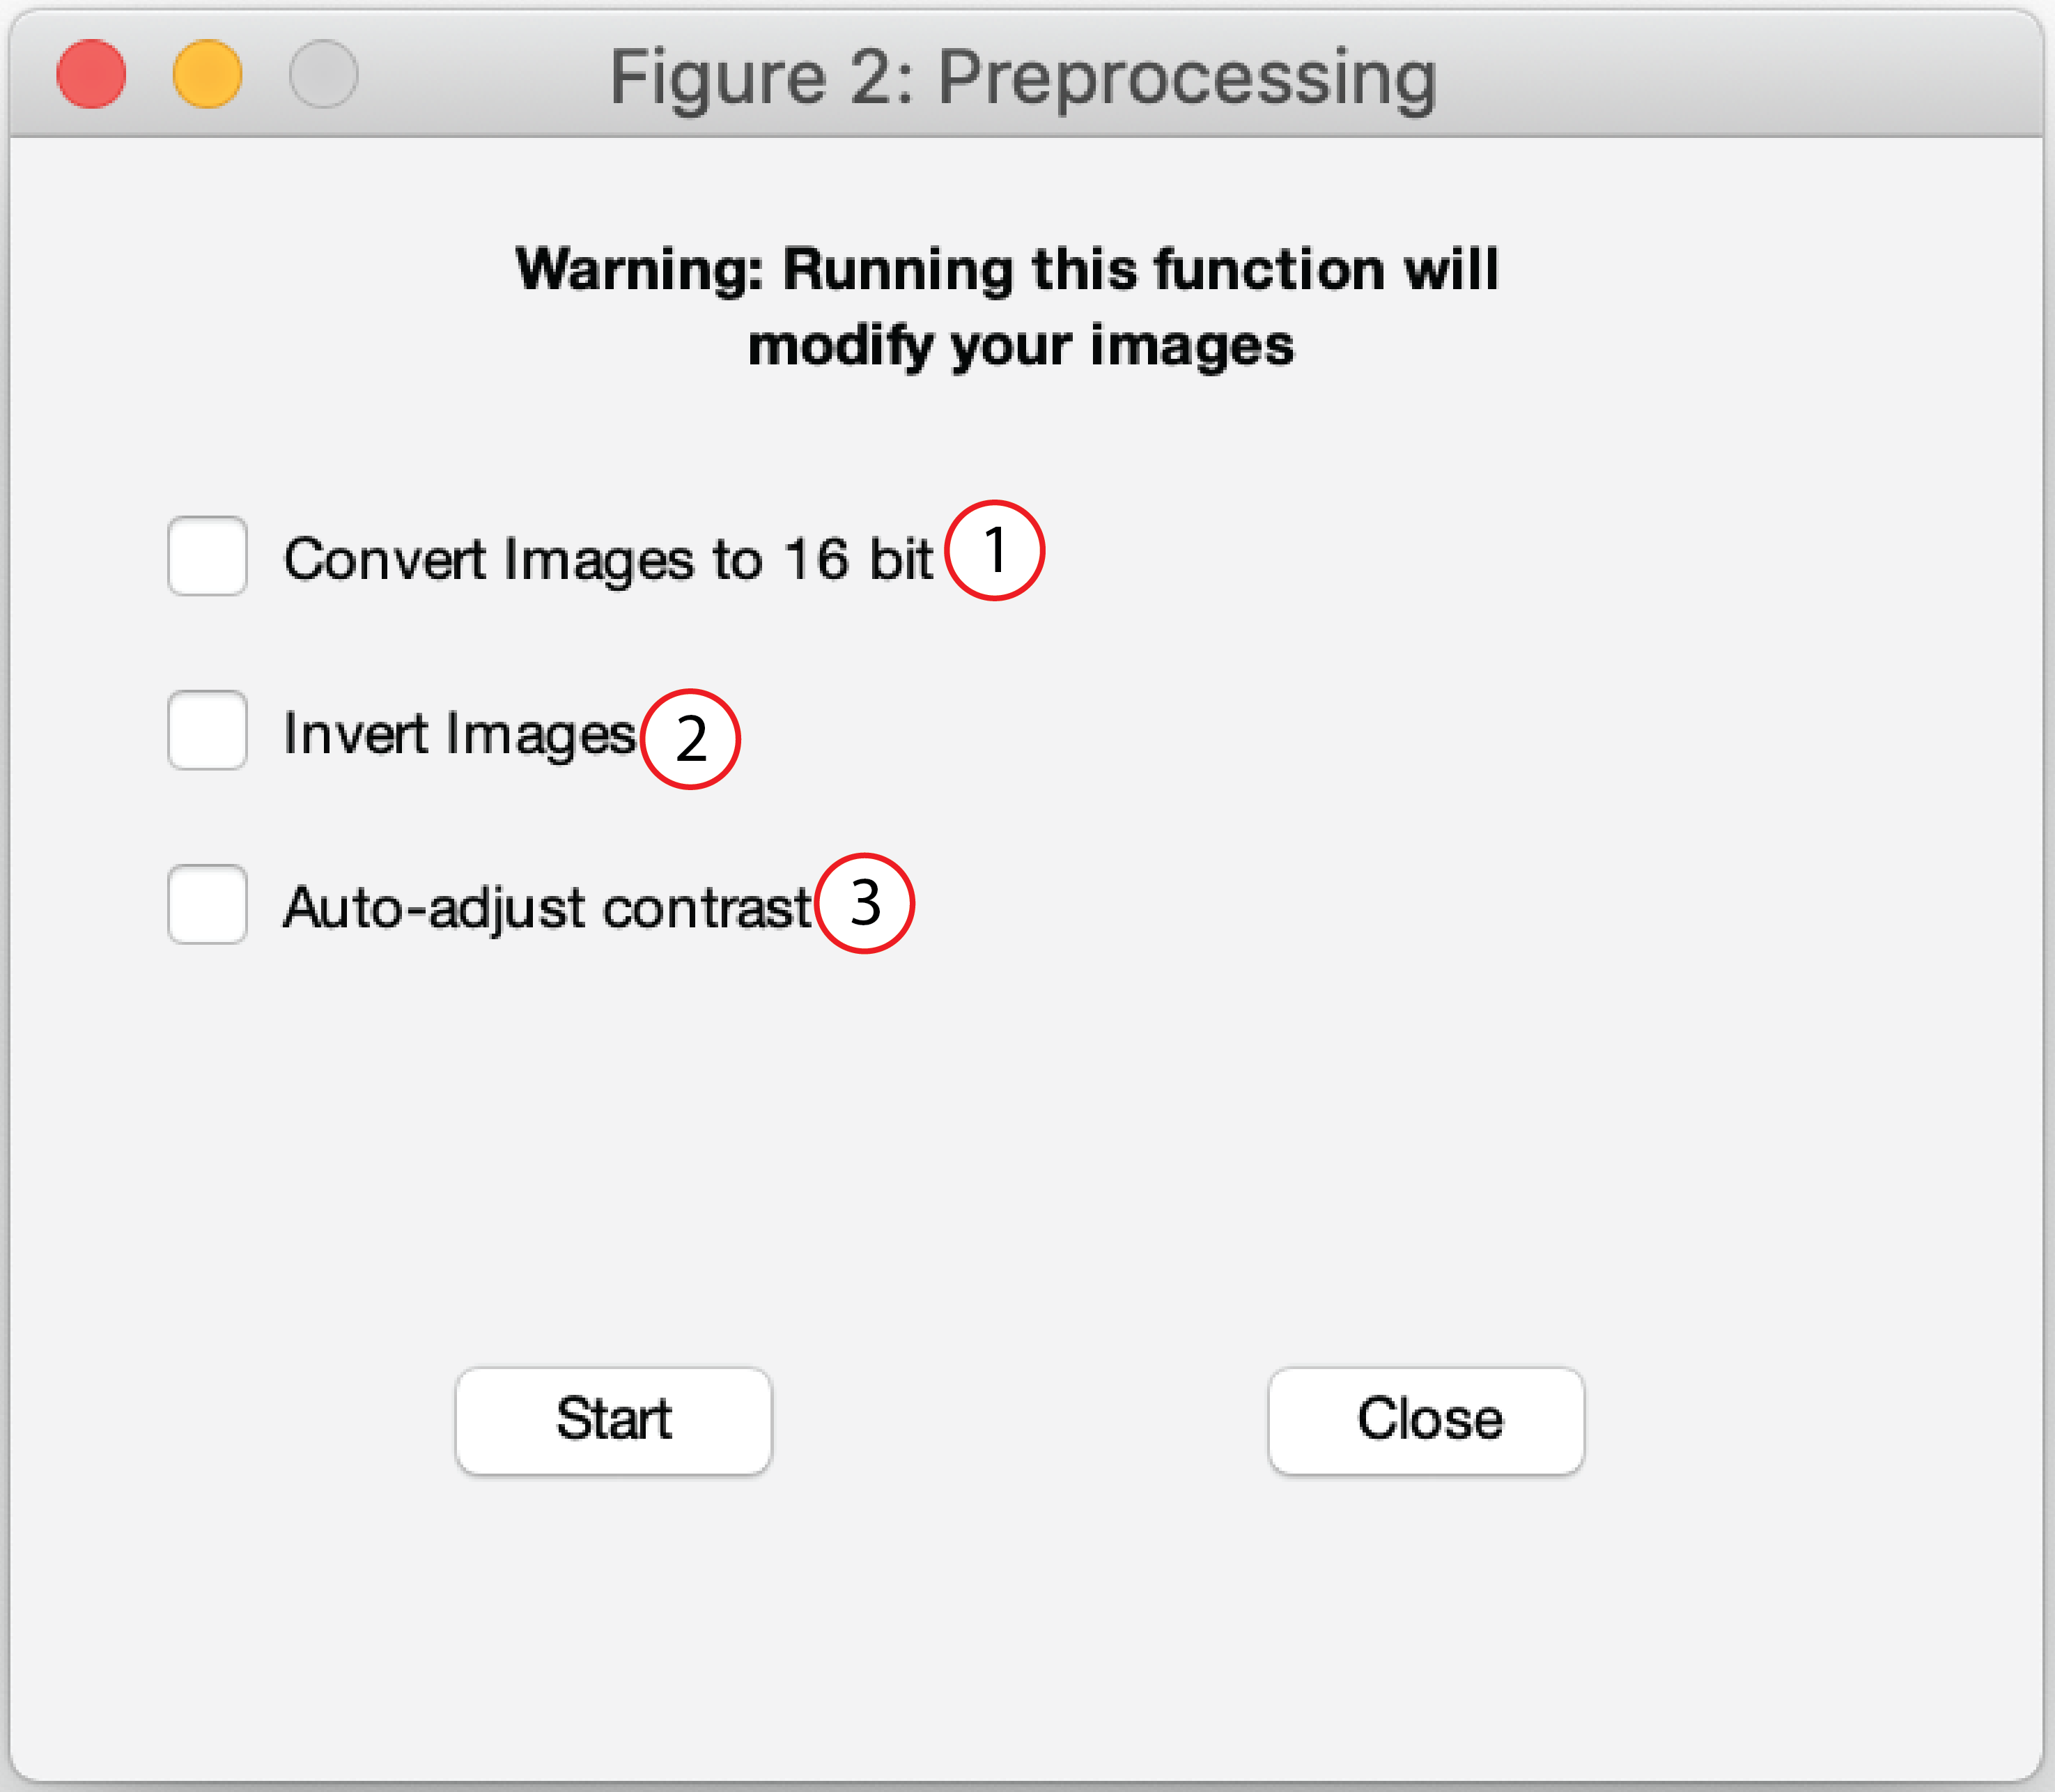
\includegraphics[scale=0.7]{screenshots/scr_preprocessing.png}
\captionsetup{singlelinecheck=off}
\caption[thing]{Preprocessing - \textbf{Warning this modifies your original image files}
\begin{enumerate}[label=\textbf{\arabic*:}, leftmargin=1.88\parindent]
\item Converts all images to 16 bit which is the necessary format for Darea. Running this multiple times will not further change your images
\item Inverts the images. This is useful when working with darkfield images. Running this a second time will restore the orginal image.
\item Automatically adjust contrast. Useful when working with images with bad contrast. Running this multiple times will further increase contrast. \emph{Warning: Running this too often may make your images unusable}
\end{enumerate}}
\end{figure}
\section{Manual Image Annotation}
\subsection{Opening images}
\label{m:openImages}
This menu is common for manual demarcation, particle detection and visualizing the results.
\begin{figure}[H]
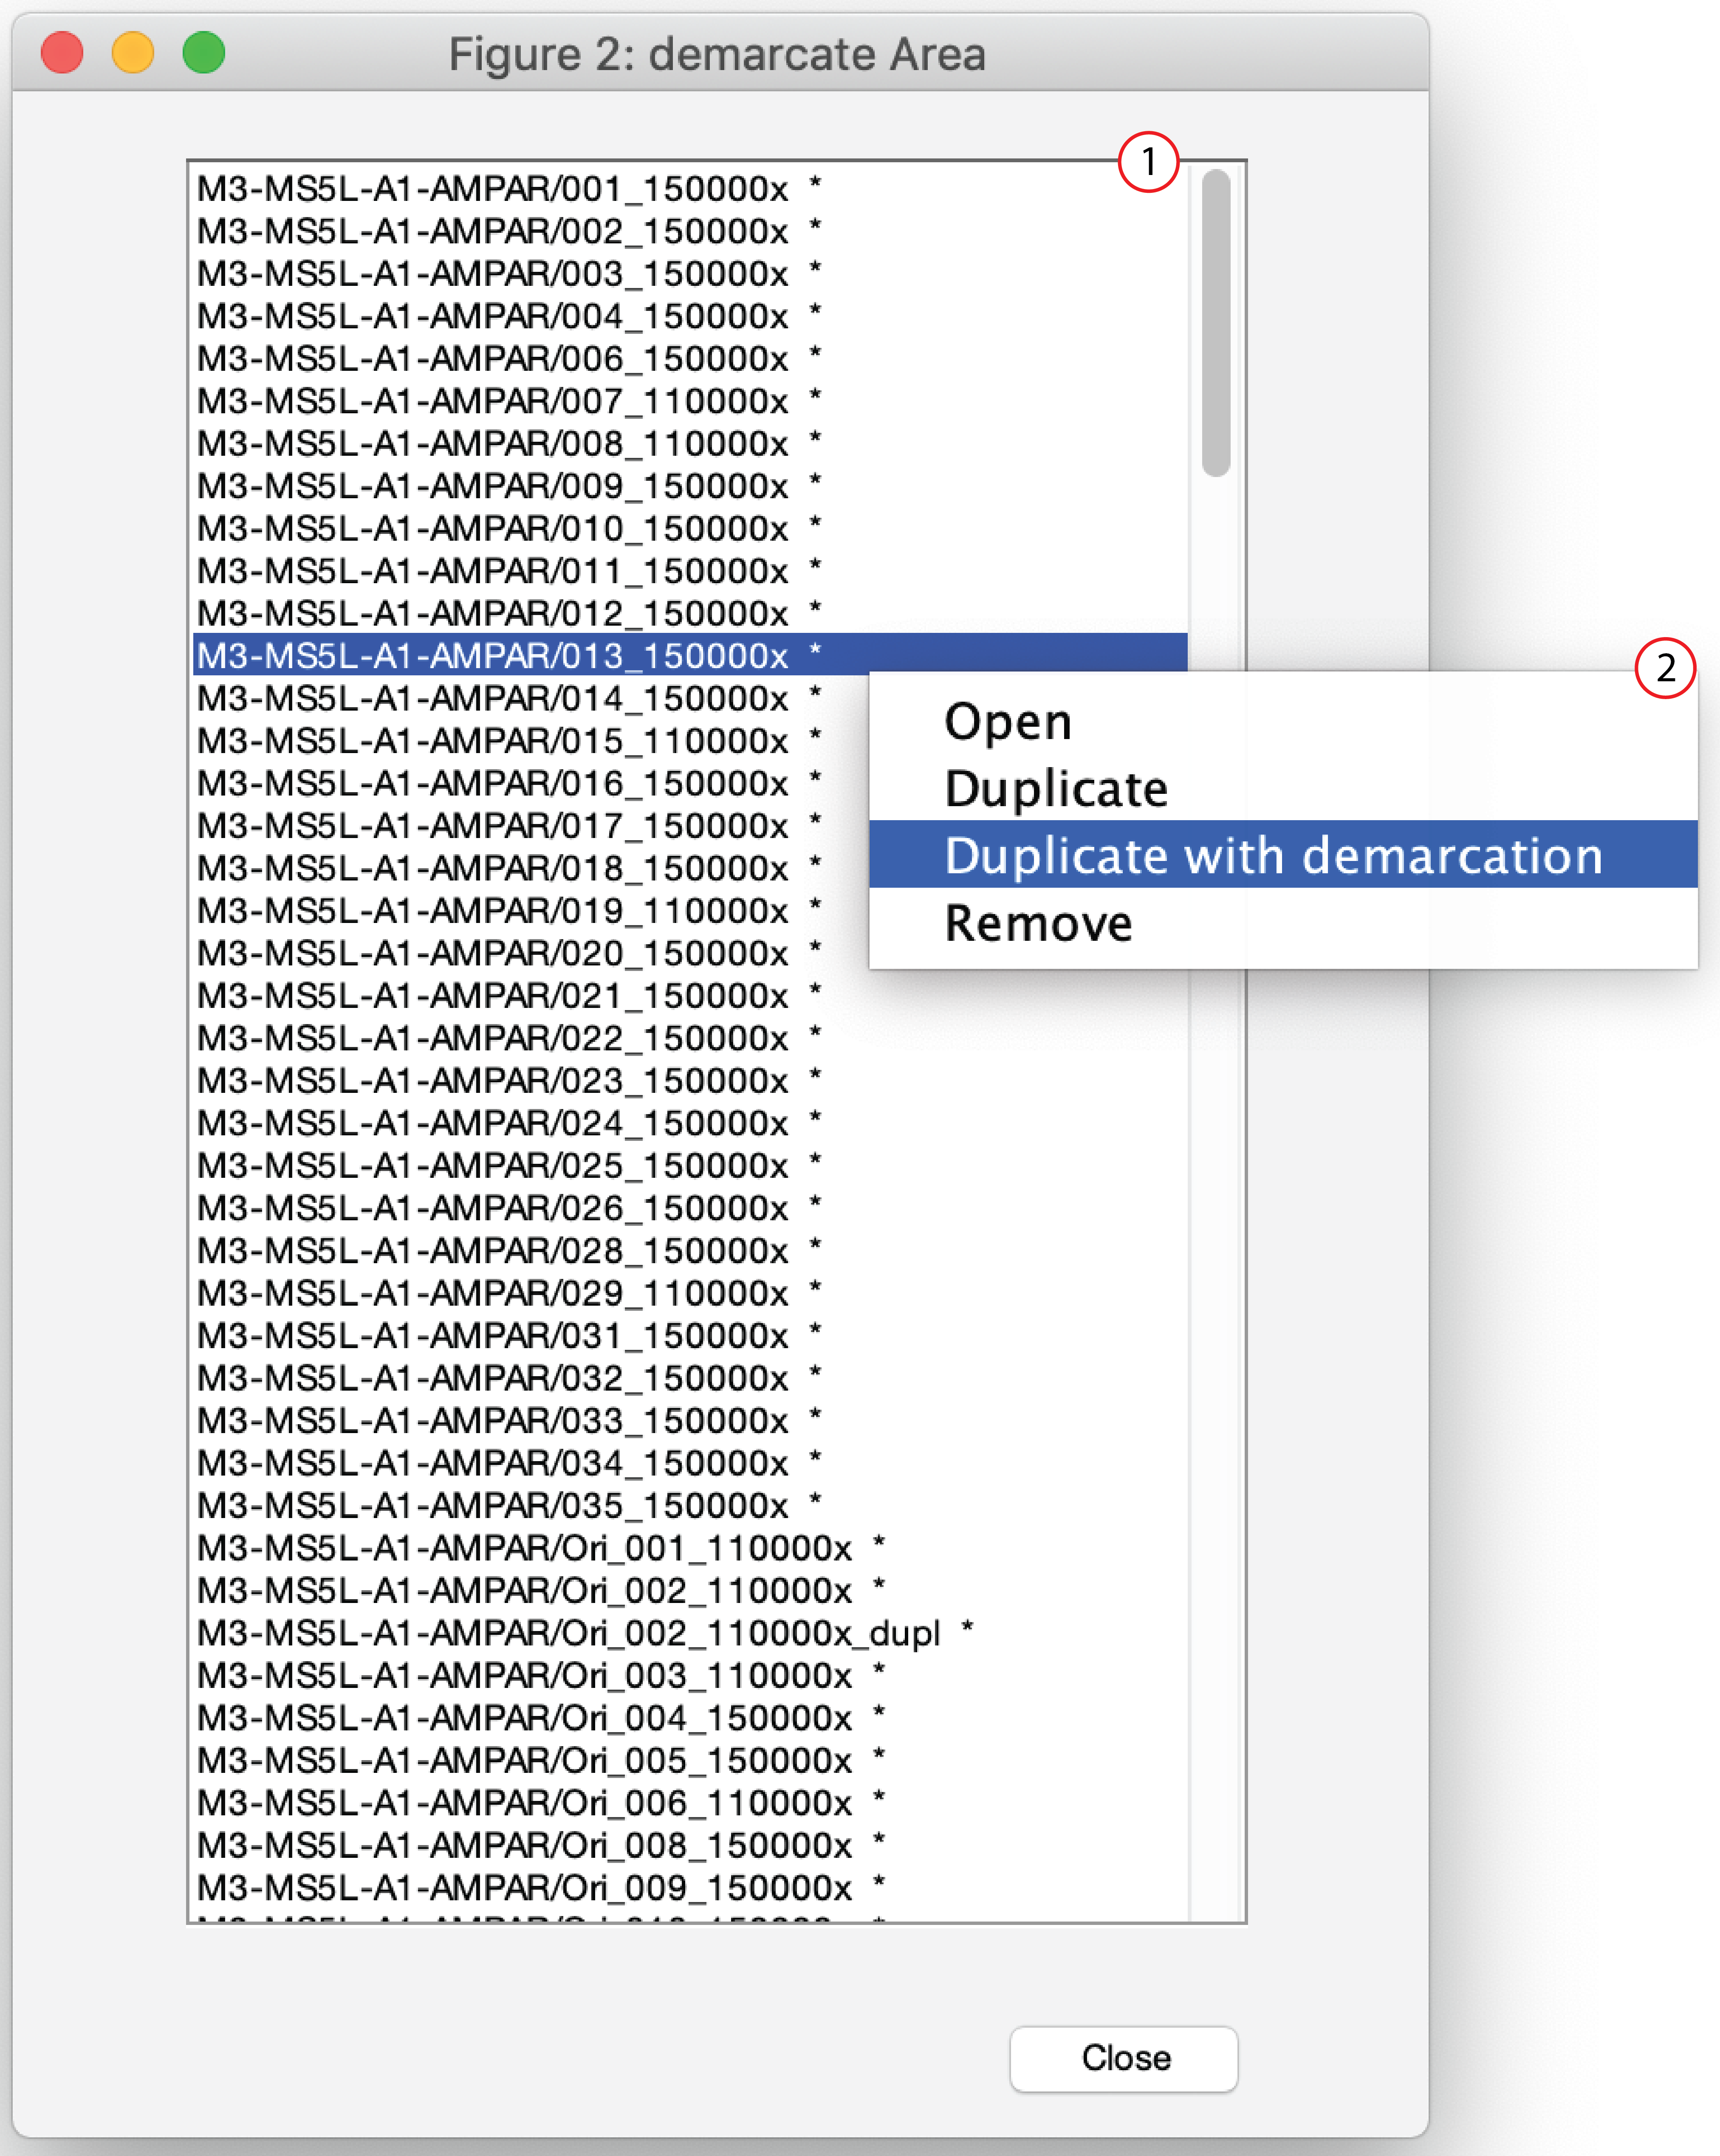
\includegraphics[scale=0.6]{screenshots/scr_openImages.png}
\captionsetup{singlelinecheck=off}
\caption[thing]{Open image
\begin{enumerate}[label=\textbf{\arabic*:}, leftmargin=1.88\parindent]
\item List of all images. Click to open image, or right click to display context menu (2). It is also possible to navigate using arrow keys and open an image by pressing enter.
\item Context Menu: "Open" will open the image (same as left clicking on it), "Duplicate" will duplicate the image. "Duplicate with demarcation" will duplicate image as well as demarcation and annotated particles. "Remove" will remove the image from the project (The image will not be deleted).
Duplicating images is useful when more than one region of interest is on the image. If more than one region if interest is annotated, it will be treated as a large discontinuous region of interest. To separate it in two region of interest, duplicate the image and demarcate one region of interest each.
\end{enumerate}}
\end{figure}

\subsection{Manual Demarcation}
\label{m:demarcate}
If more than one region if interest is demarcated, it will be treated as a large discontinuous region of interest. To separate it in two region of interest, duplicate the image and demarcate one region of interest each.
\begin{figure}[H]
\includegraphics[width=\linewidth]{screenshots/scr_Dem_Polygon.png}
\captionsetup{singlelinecheck=off}
\caption[thing]{Manual demarcation
\begin{enumerate}[label=\textbf{\arabic*:}, leftmargin=1.88\parindent]
\item Overview image. Blue square outlines the regions displayed in (2) and can be moved and scaled.
\item Zoomed region. Clicking into this image allows you to create a polygon around your area of interest
\item Coordinates of the zoomed region. Can be manually edited to move blue rectangle to the described position
\item Rotate image 90°. All demarcations and annotated particle will rotate accordingly.
\item Length of the image shown in (2) in nm. Decrease the value to zoom in or increase to zoom out.
\item Select what should be displayed in the right panel (2). In this case the original image is displayed, which allows you to manually demarcate a region of interest (ROI). If a demarcation has been saved before, you can display it by choosing "saved Component".
\item When pressed click in (2) to measure distance between two points
\item When pressed clicking in (2) will allow to draw a freehand demarcation. After finishing your freehand drawing, click freehand again to convert it to a polygon (neccessary for saving the demarcation).
\item Convert your demarcation into a component that can be further modified (see Fig.\ref{fig:dSaved}. Clicking this button is equivalent to saving, closing, reopening and selecting "saved Component" in (6).
\item Clears the polygon
\item Removes the last point of the polygon. Can be also done by pressing backspace
\item Save the demarcation
\item Close without saving
\end{enumerate}}
\label{fig:dPoly}
\end{figure}
\begin{figure}[H]
\includegraphics[width=\linewidth]{screenshots/scr_Dem_saved.png}
\captionsetup{singlelinecheck=off}
\caption[thing]{Manual demarcation
Please refer to \ref{fig:dPoly} for buttons already described there.
\begin{enumerate}[label=\textbf{\arabic*:}, leftmargin=1.88\parindent]
\item Zoomed image showing the components. Clicking on a component here will select this one and discard other components. That component can be then further refined (see Fig.\ref{fig:dFinalize})
\item Select what should be displayed in the right panel (1). In this case the saved Component is displayed, which allows you to modify it or select a particular connected component by clicking on it.
\item When pressed, clicking on (1) will draw a polygon. Clicking add again will add the selected polygon as a component
\item When pressed, clicking on (1) will draw a polygon. Clicking remove again will remove the selected polygon from the component.
\item When pressed, clicking on (1) will draw a line. Clicking trim again will remove this line from the component. Useful for separating one component into two.
\item When pressed, two components can be selected in (1). They will then be connected by a thin line where the two components are closest.
\item Change the brightness of the background which is not part of a component
\end{enumerate}}
\label{fig:dSaved}
\end{figure}
\begin{figure}[H]
\includegraphics[width=\linewidth]{screenshots/scr_Dem_finalize.png}
\captionsetup{singlelinecheck=off}
\caption[thing]{Manual demarcation. Please refer to Fig.\ref{fig:dPoly} for buttons already described there.
\begin{enumerate}[label=\textbf{\arabic*:}, leftmargin=1.88\parindent]
\item Select what should be displayed in the right panel (1). In this case a single connected component is displayed, which allows you to perform some automated finalizing steps like closing the structure or filling holes. Clicking on (5) will make it a new component which allows further manual modification.
\item This closes the region of interest with a radius of 7.5 nm. Demarcated points closer than 15 nm will be connected. This will lead to the removal of small holes and a smoother outline.
\item Fills any holes within the component
\item Makes the component modifiable again (see Fig.\ref{fig:dSaved})
\end{enumerate}}
\label{fig:dFinalize}
\end{figure}
\subsection{Manual particle detection}
\label{m:particles}
\begin{figure}[H]
\includegraphics[width=\linewidth]{screenshots/scr_Particles.png}
\captionsetup{singlelinecheck=off}
\caption[thing]{Manual particle labeling. Please refer to Fig.\ref{fig:dPoly} for buttons already described there.
\begin{enumerate}[label=\textbf{\arabic*:}, leftmargin=1.88\parindent]
\item Click on a particle to annotate it. Automatically, a black circle near where you clicked will be detected and annotated. So it is not necessary to precisely click the center of a particle
\item Select the particle size you are annotating
\item Measured diameter of the last annotated particle (depending on image contrast, this may be more or less accurate)
\item Sensitivity of the circle detection algorithm. Higher values will lead to more false positives, smaller values to more false negatives. If you try to click on a particle, but none is detected, try increasing this value.
\item Margin around the particle size, e.g. if the expected particle diameter is 6 nm and the margin is 2, particles between 4 and 8 nm will be accepted.
\item When selected clicking in (1) will annotate the particle with center exactly where you clicked. 
\item Whether or not to show particle labels. When correcting automatic annotation, quickly switching labels on and off facilitates searching for false positives. 
\item Automated particle detection of the selected size on this image. Margin and sensitivity are taken into account.
\item The classifier used for automated detection. Please refer to \ref{m:trainPart} for details. 
\end{enumerate}}
\label{fig:particles}
\end{figure}
\section{Automated demarcation and particle annotation}
\label{m:auto}
\begin{figure}[H]
\includegraphics[scale=0.5]{screenshots/scr_prediction.png}
\captionsetup{singlelinecheck=off}
\caption[thing]{Automated demarcation and particle prediction
\begin{enumerate}[label=\textbf{\arabic*:}, leftmargin=1.88\parindent]
\item Whether or not to predict demarcation
\item Which feature should be detected. Refer to \ref{m:trainDem} for details.
\item Should existing demarcations be overwritten?
\item Whether or not particles should be automatically annotated
\item Should existing annotations be overwritten?
\item Should the prediction be limited to the demarcation only (much faster and therefore highly recommended).
\item Sensitivity and size margin of the circle detection algorithm. Please refer to Fig.\ref{fig:particles} for more details.
\item The classifier used for automated detection. Please refer to \ref{m:trainPart} for details. 

\end{enumerate}}
\end{figure}
\section{Analysis}
\subsection{Running Analysis}
\label{m:analysis}
\begin{figure}[H]
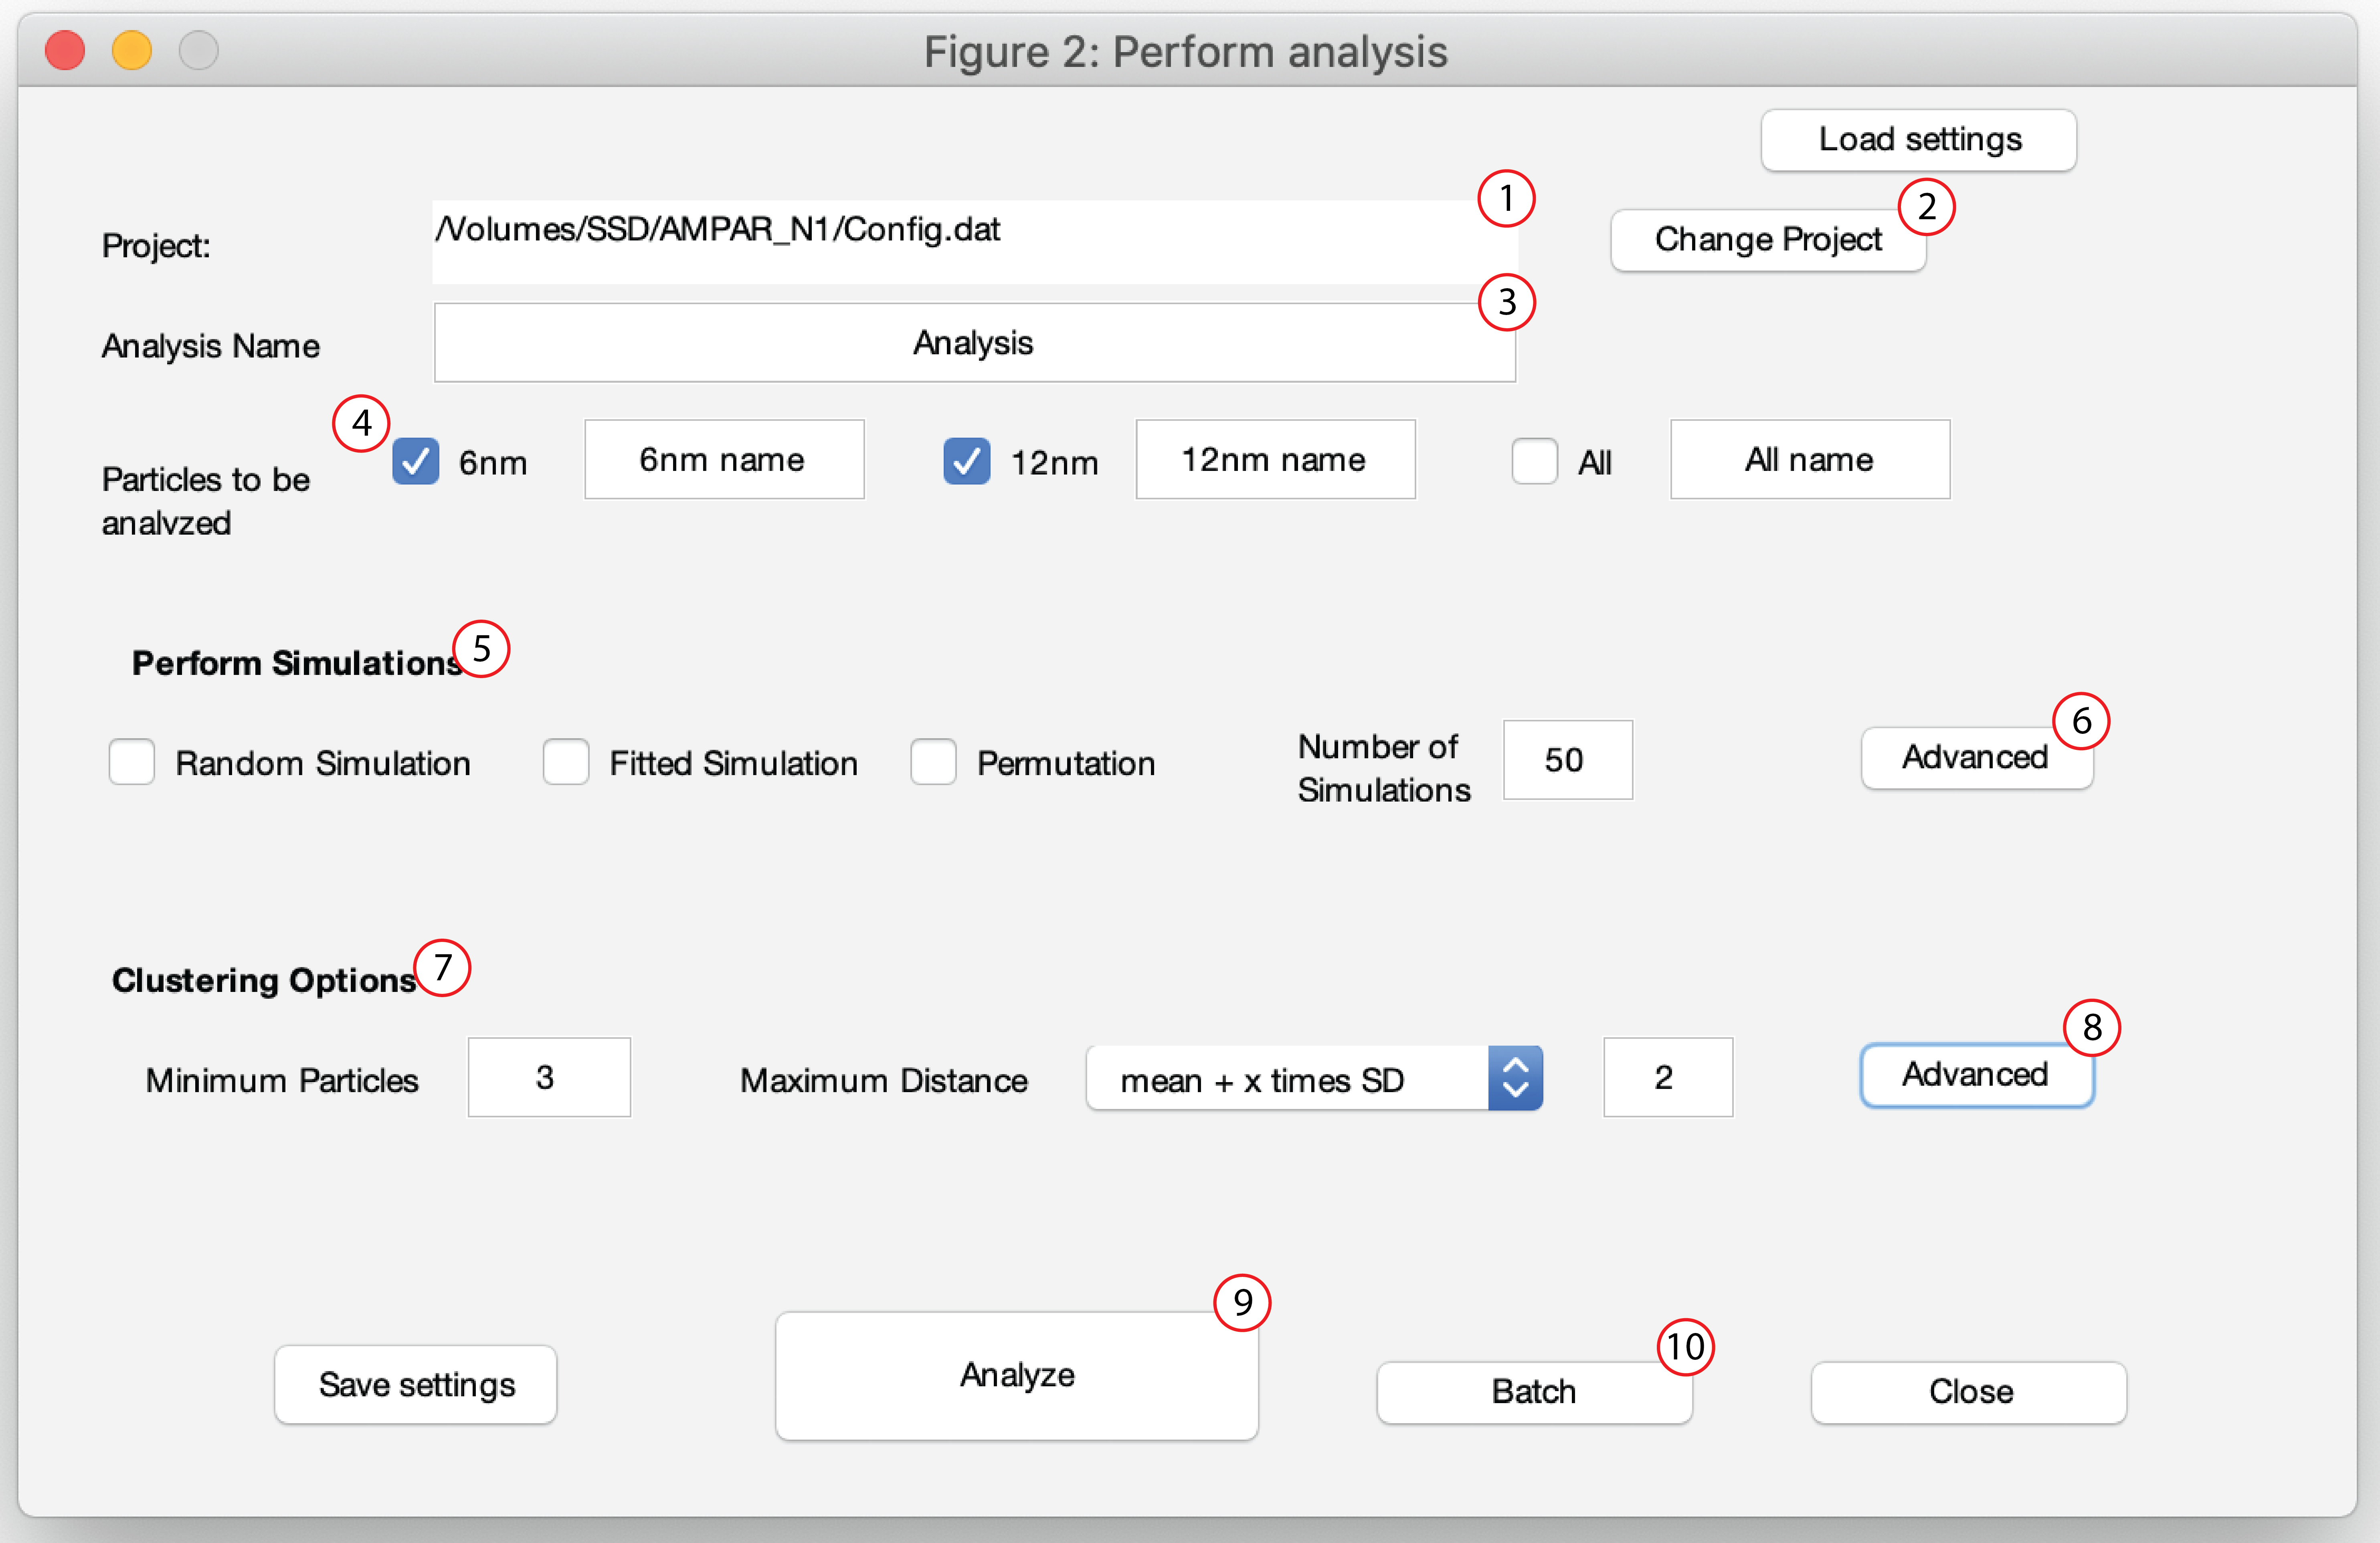
\includegraphics[scale=0.55]{screenshots/scr_Analysis.png}
\captionsetup{singlelinecheck=off}
\caption[thing]{Analysis
\begin{enumerate}[label=\textbf{\arabic*:}, leftmargin=1.88\parindent]
\item Path to the project file
\item Change to a different project
\item Name of this analysis. Within the same project, analyses with different parameters (e.g. which simulations should be run) can be performed. They should then have different names to allow for easy distinction
\item Which particle sizes to analyze. You may give each particle size a name to facilitate interpretation of resulting data tables. "All" means all particle sizes are analyzed irrespective of size (in addition to any ticked sizes).
\item Options for Monte-Carlo simulations (see \ref{m:simulations}
\item Advanced settings for simulations (see Fig.\ref{fig:SimOptions})
\item Clustering options (see \ref{m:clusters})
\item Advanced settings for clusterings (see Fig.\ref{fig:ClusterOptions})
\item Start analysis
\item Sometimes you may want to run multiple different analyses. Pressing batch designates your current input for analysis, then reopens this window. You may then specify your next analysis to run. After you finished setting up each analysis, press Analyze (9) to run all analyses at once.
\end{enumerate}}
\label{fig:analysis}
\end{figure}
\subsubsection{Monte-Carlo Simulations}
\label{m:simulations}
There are 3 kinds of simulations: Random, fitted and permutations. \\ Random simulation: The same number of particles as in the original image is redistributed in the region of interest. Each pixel as the same probability of becoming the center of a particle. Particles need to be some minimum distance from each other. \\ Fitted simulation: First a random simulation is performed, than it is checked if the particle distribution is appropriate (see Fig. \ref{fig:SimOptions} (2)). If so it is accepted, if not a random particle is randomly redistributed and it is checked if the new simulation is closer to acceptable than the old. If so, it is kept, otherwise it is reverted to the previous situation. This is repeated until the distribution is appropriate. \\ For both random and fitted simulation, only particles of one size are simulated at the same time (i.e. different simulations will be created for simulated 5nm and simulated 10 nm particles). \\ Permutation: Particle identities are randomly reassigned (e.g. if there are 2 5nm particles and 3 10nm particles, 2 particles will be randomly picked to become 5nm and the others become 10nm).
\begin{figure}[H]
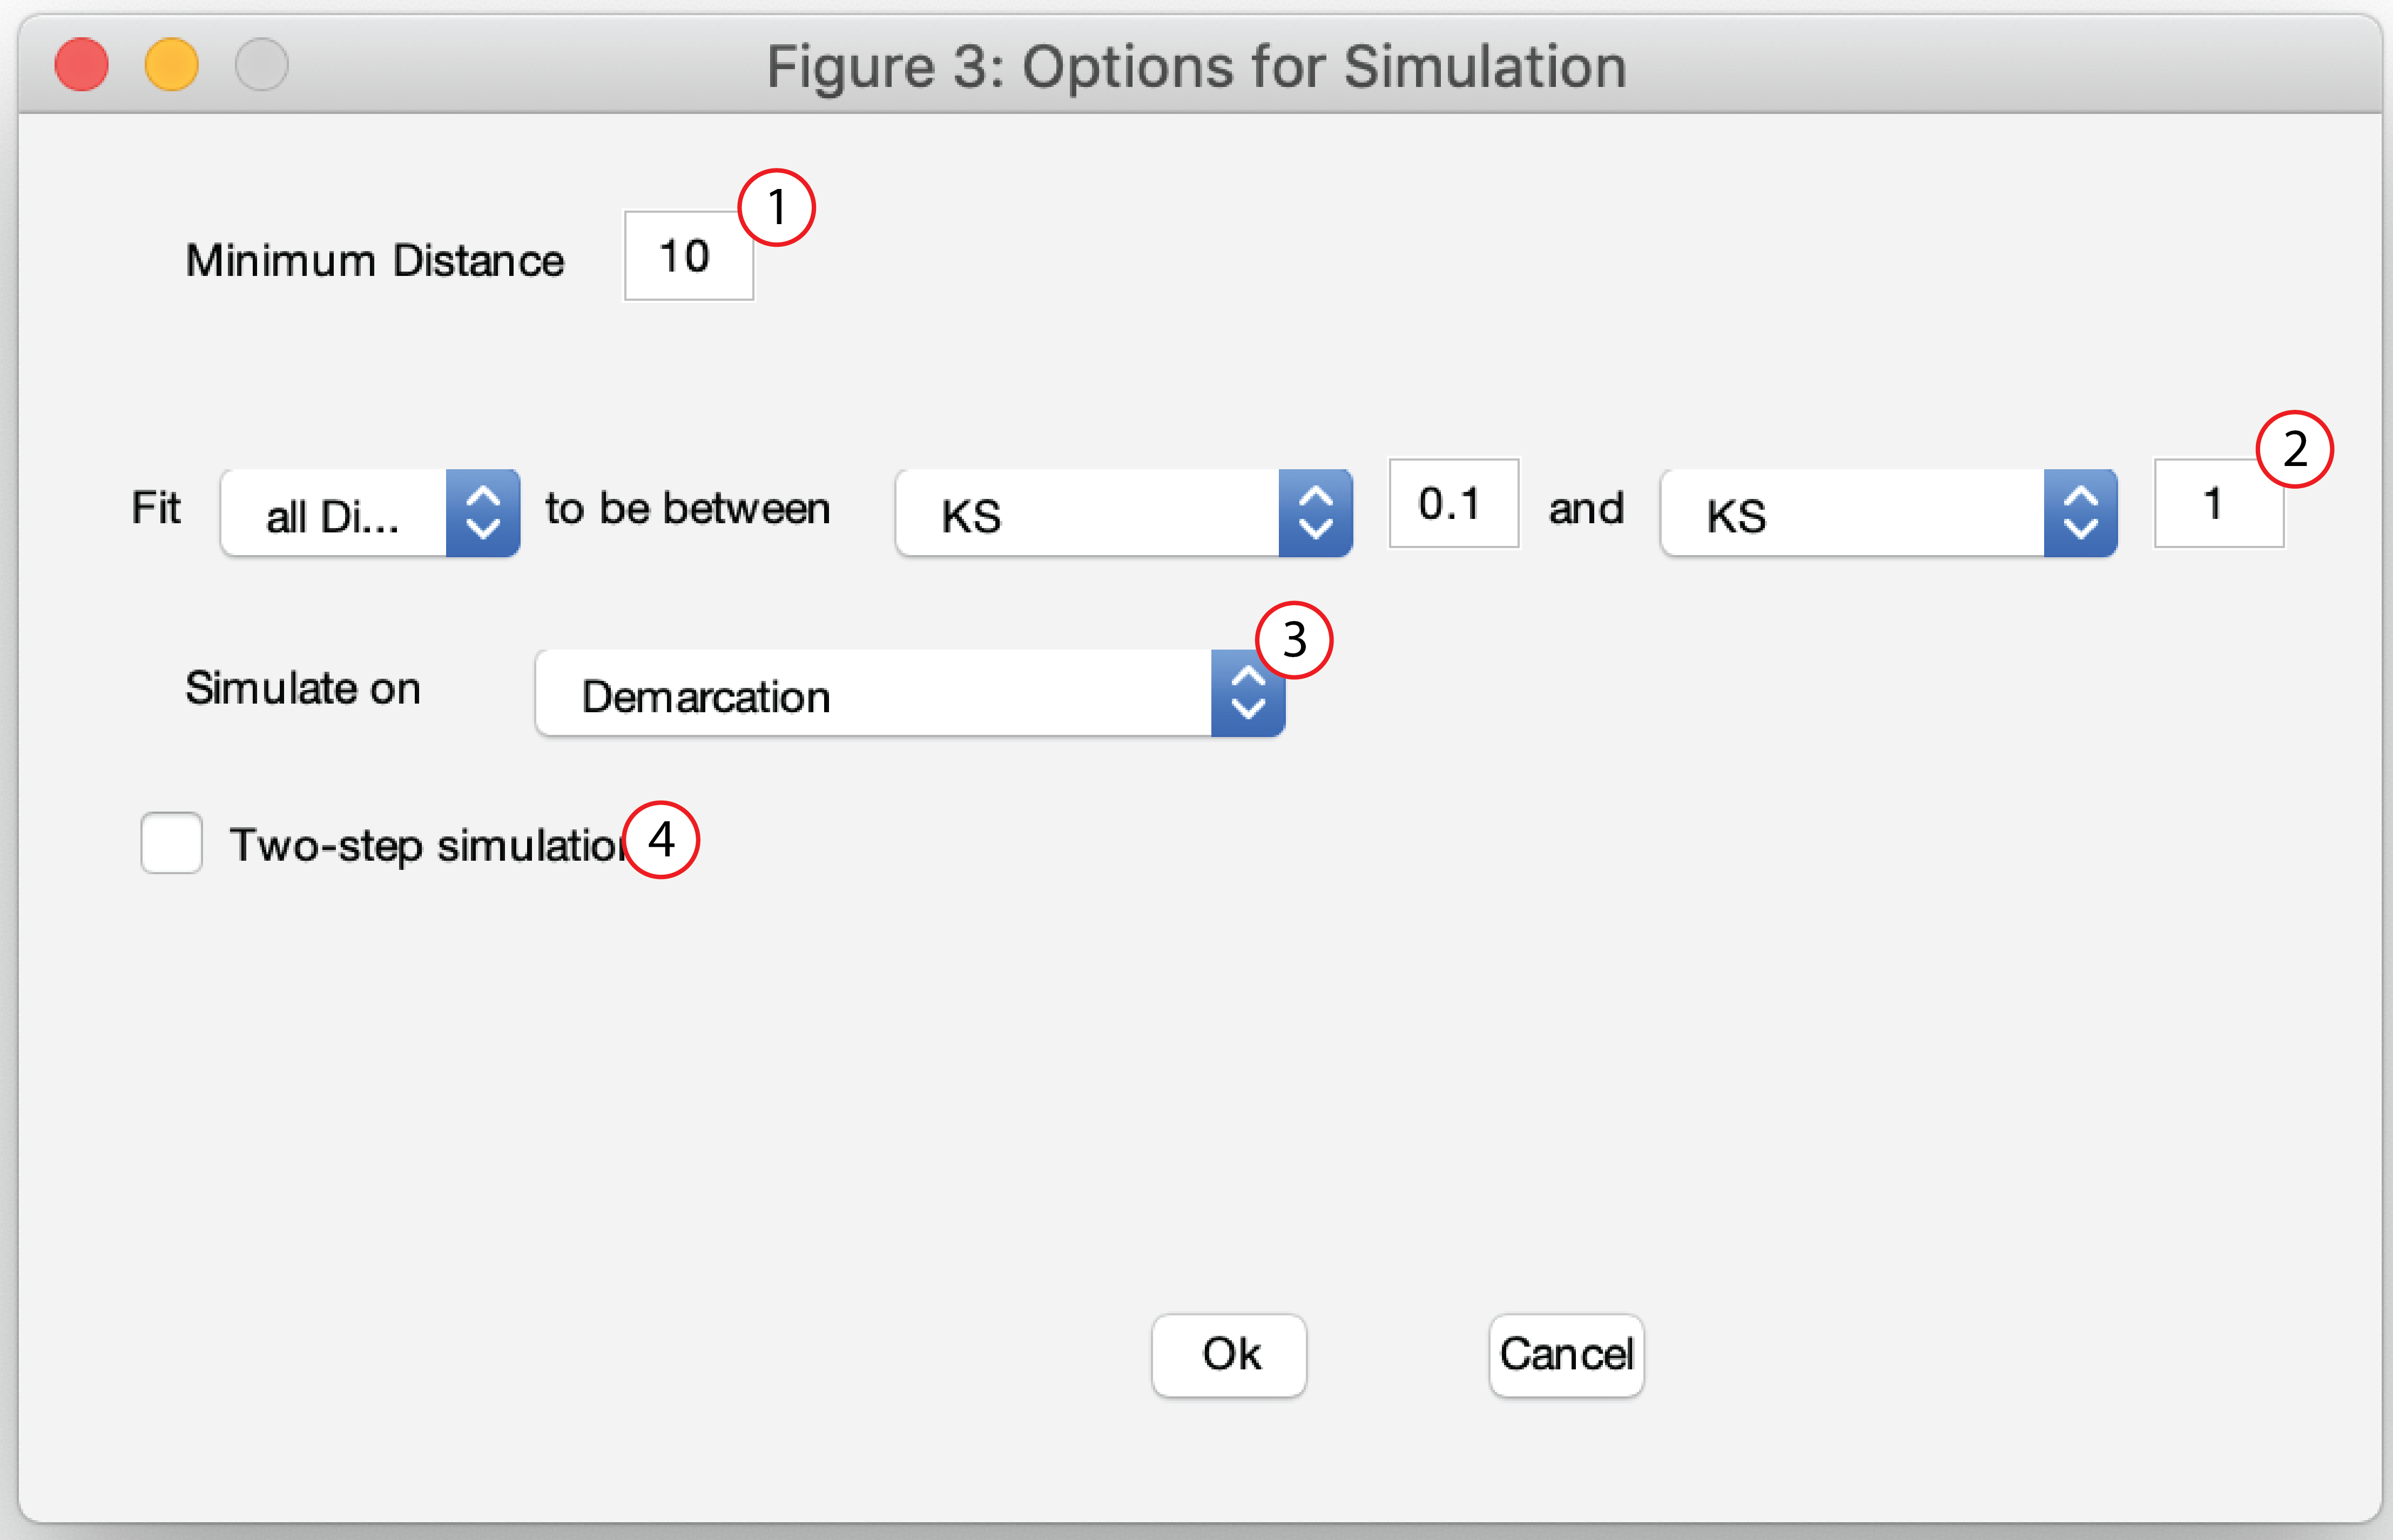
\includegraphics[scale=0.55]{screenshots/scr_SimOptions.png}
\captionsetup{singlelinecheck=off}
\caption[thing]{Simulation Options
\begin{enumerate}[label=\textbf{\arabic*:}, leftmargin=1.88\parindent]
\item  Minimum distance between two particles
\item Describes when a fitted simulation is appropriate. In this case all Distances between particles will be compared between real and simulated using a Kolmogorov-Smirnov (KS) test. If the p-Value is between 0.1 and 1, the simulation is accepted.
\item Whether to simulated particles should be distributed only on demarcation or on demarcation + outer rim
\item If clicked, rather than distributing particles immediately, first epitopes (i.e what you were labeling for) are randomly distributed. In a second step particles are then redistributed a random distance (between 0 and a specified distance) at a random angle away from the epitope.
\end{enumerate}}
\label{fig:SimOptions}
\end{figure}
\subsubsection{Clusters}
\label{m:clusters}
Clusters are composed of a minimum number of particles which are closer to each other than some minimum distance. For these clusters of particles, several parameters will be computed: Cluster Area, number of particle per cluster, number of clusters per image, density of particles in a cluster, distance between clusters, overlap between clusters. The minimum number of particles that can be specified is 3 (because clusters smaller than that would not have an area, as they would just be a line between particles). The maximum distance between particles of the same clusters can be specified either in nm, or can be calculated from average NND. In the example above, this maximum distance is calculated as mean + 2*SD of the NND.
\begin{figure}[H]
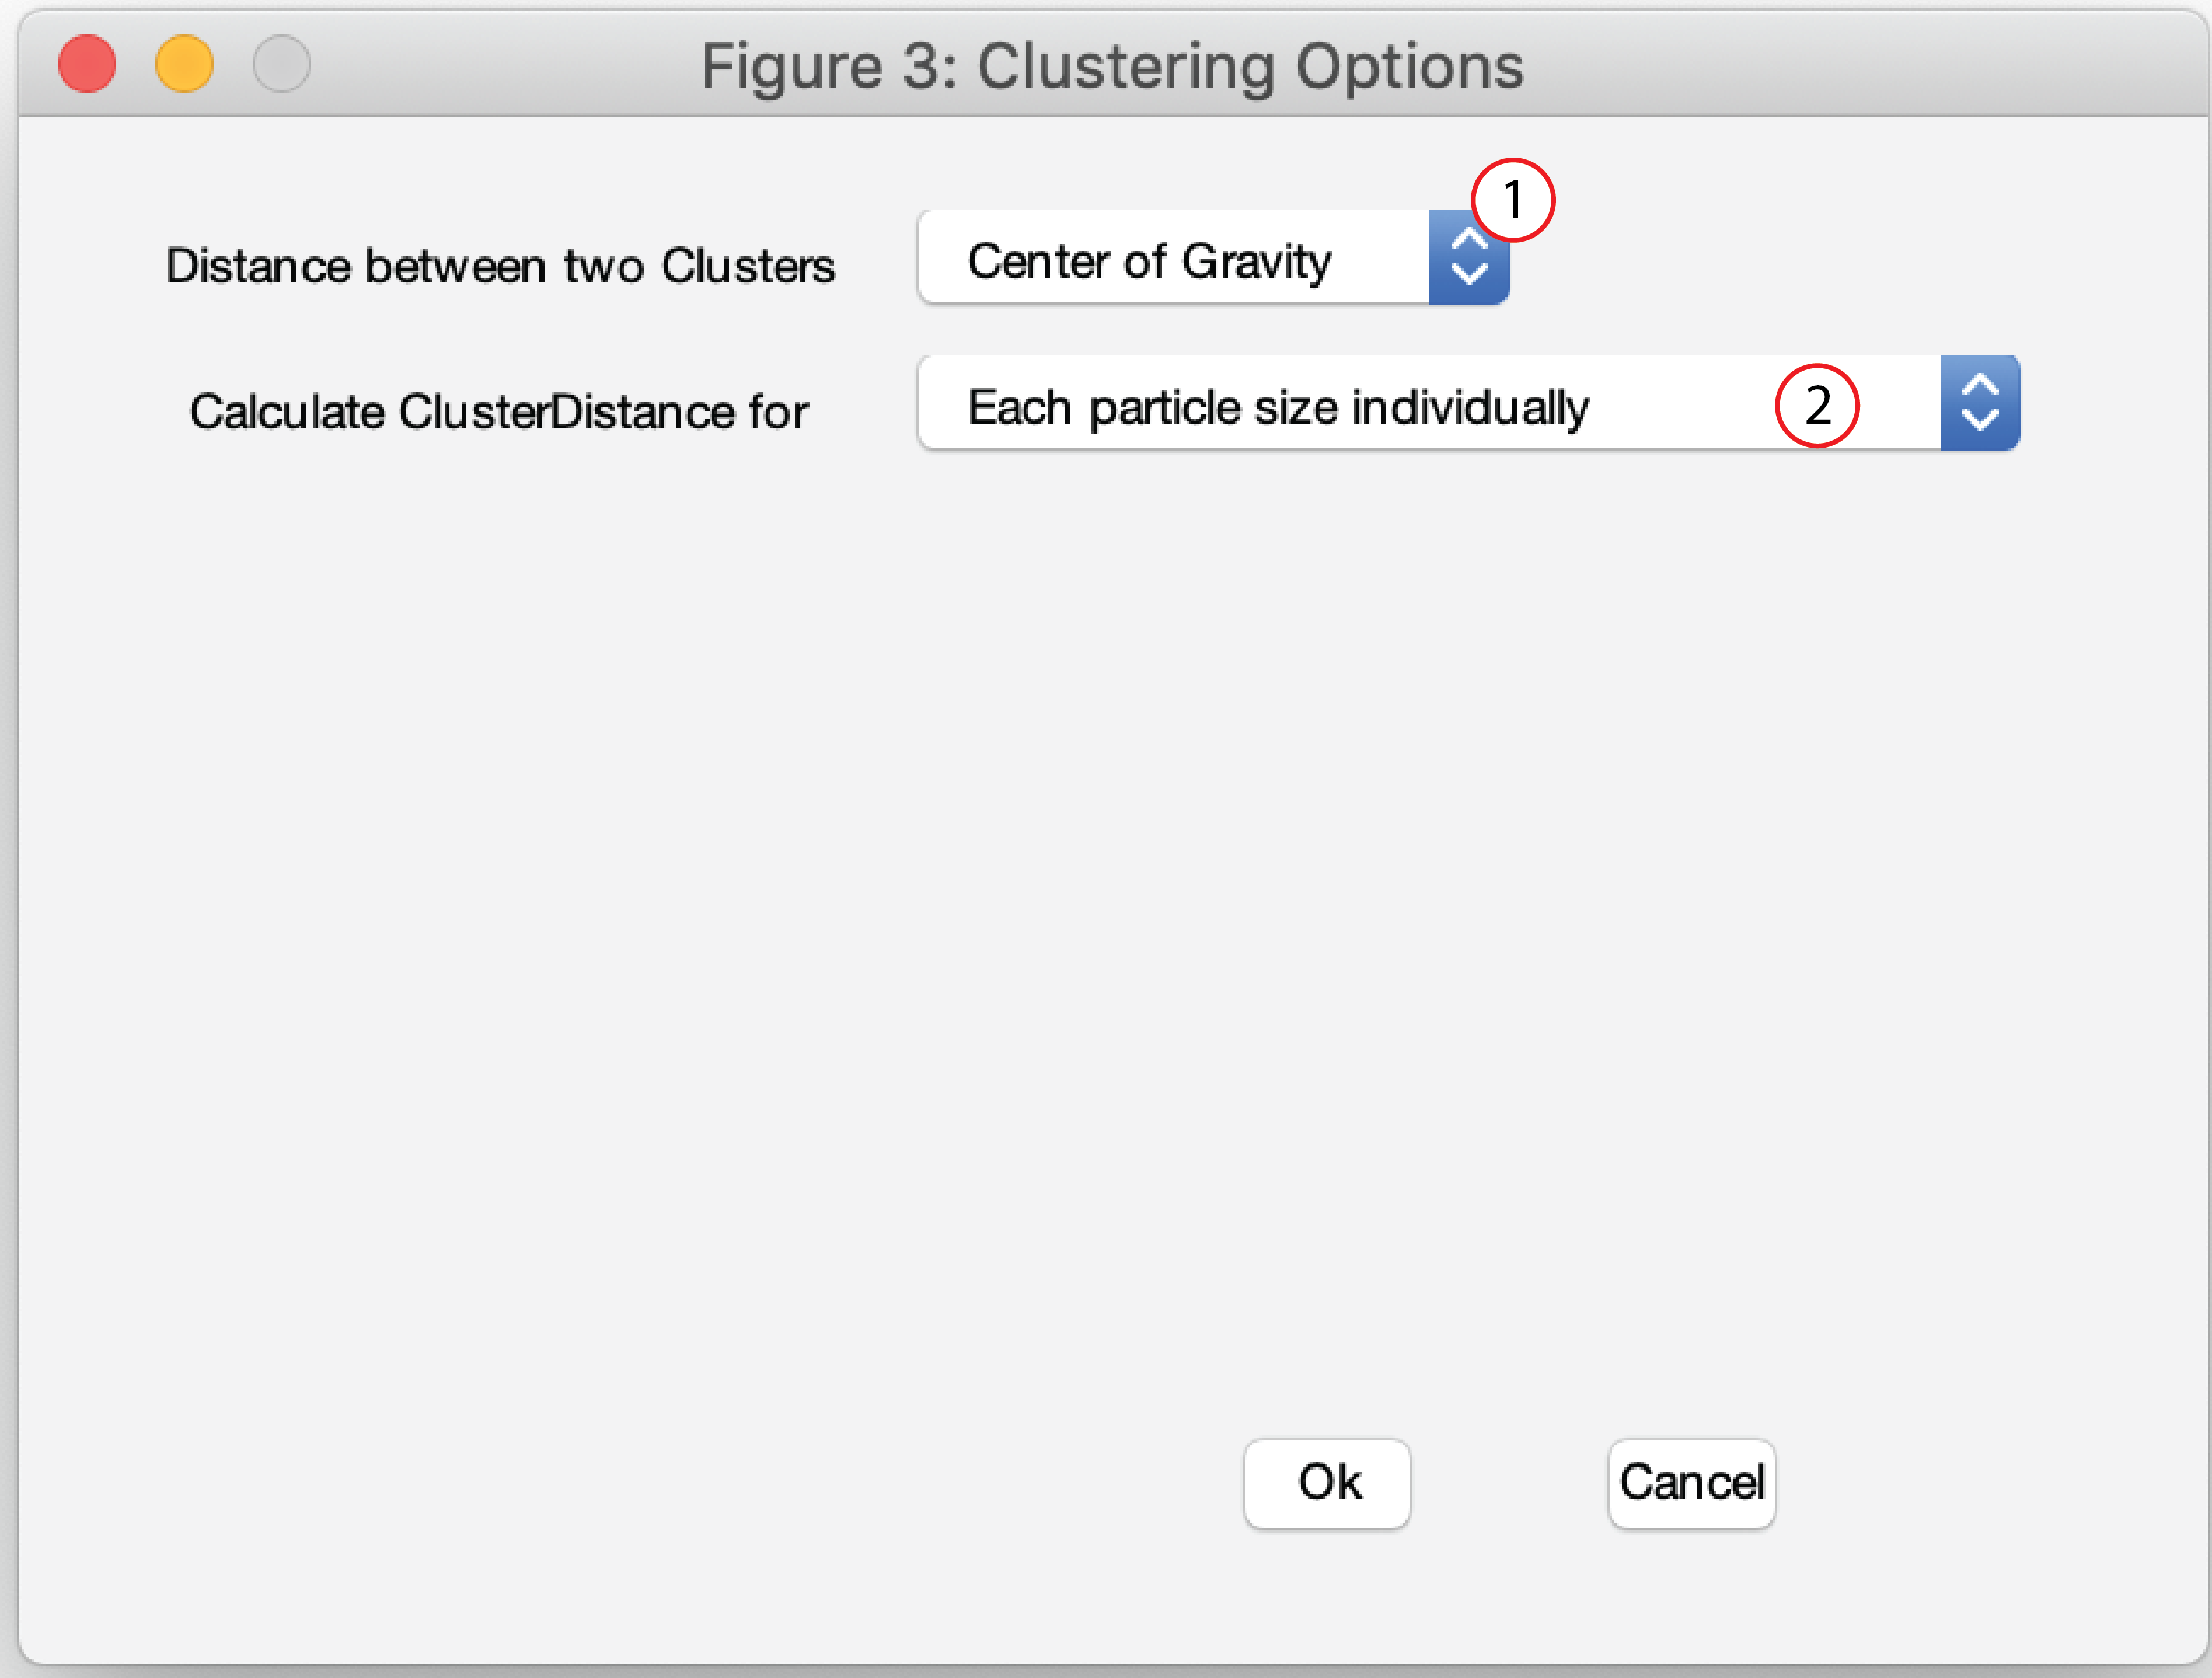
\includegraphics[scale=0.55]{screenshots/scr_ClusterOptions.png}
\captionsetup{singlelinecheck=off}
\caption[thing]{Clustering Options
\begin{enumerate}[label=\textbf{\arabic*:}, leftmargin=1.88\parindent]
\item How distance between two clusters should be measured. \\The possibilities are: "Center of Gravity" -> Distance between the two cluster's center of gravities.\\ "Particle to Particle" -> Distance between the two nearest particle of the clusters.\\ "Outline to Outline" -> Distance between the two nearest points of the cluster outlines (Outline is specified as convex hull of all particle centers of the cluster).
\item If cluster distance is not fixed in nm, but calculated from NND. From what should it be calculated?\\ The Options are: \\"All groups and particle sizes together" -> mean and SD of NND is calculated from pooled data regardless of particle size or group. \\"Each particle size individually" -> mean and SD is calculated for each particle size separately. That means different particle sizes will have different maximum distances for clustering. \\"Each group individually" -> mean and SD is calculated for each group individually. Different particle sizes are pooled. \\"Each group and particle size individually" -> mean and SD is calculated for each group and particle size individually. If groups should calculated individually, a selection will appear where you can select which groupings are relevant.
\end{enumerate}}
\label{fig:ClusterOptions}
\end{figure}
\subsection{Making tables and figures}
\label{m:figures}
\begin{figure}[H]
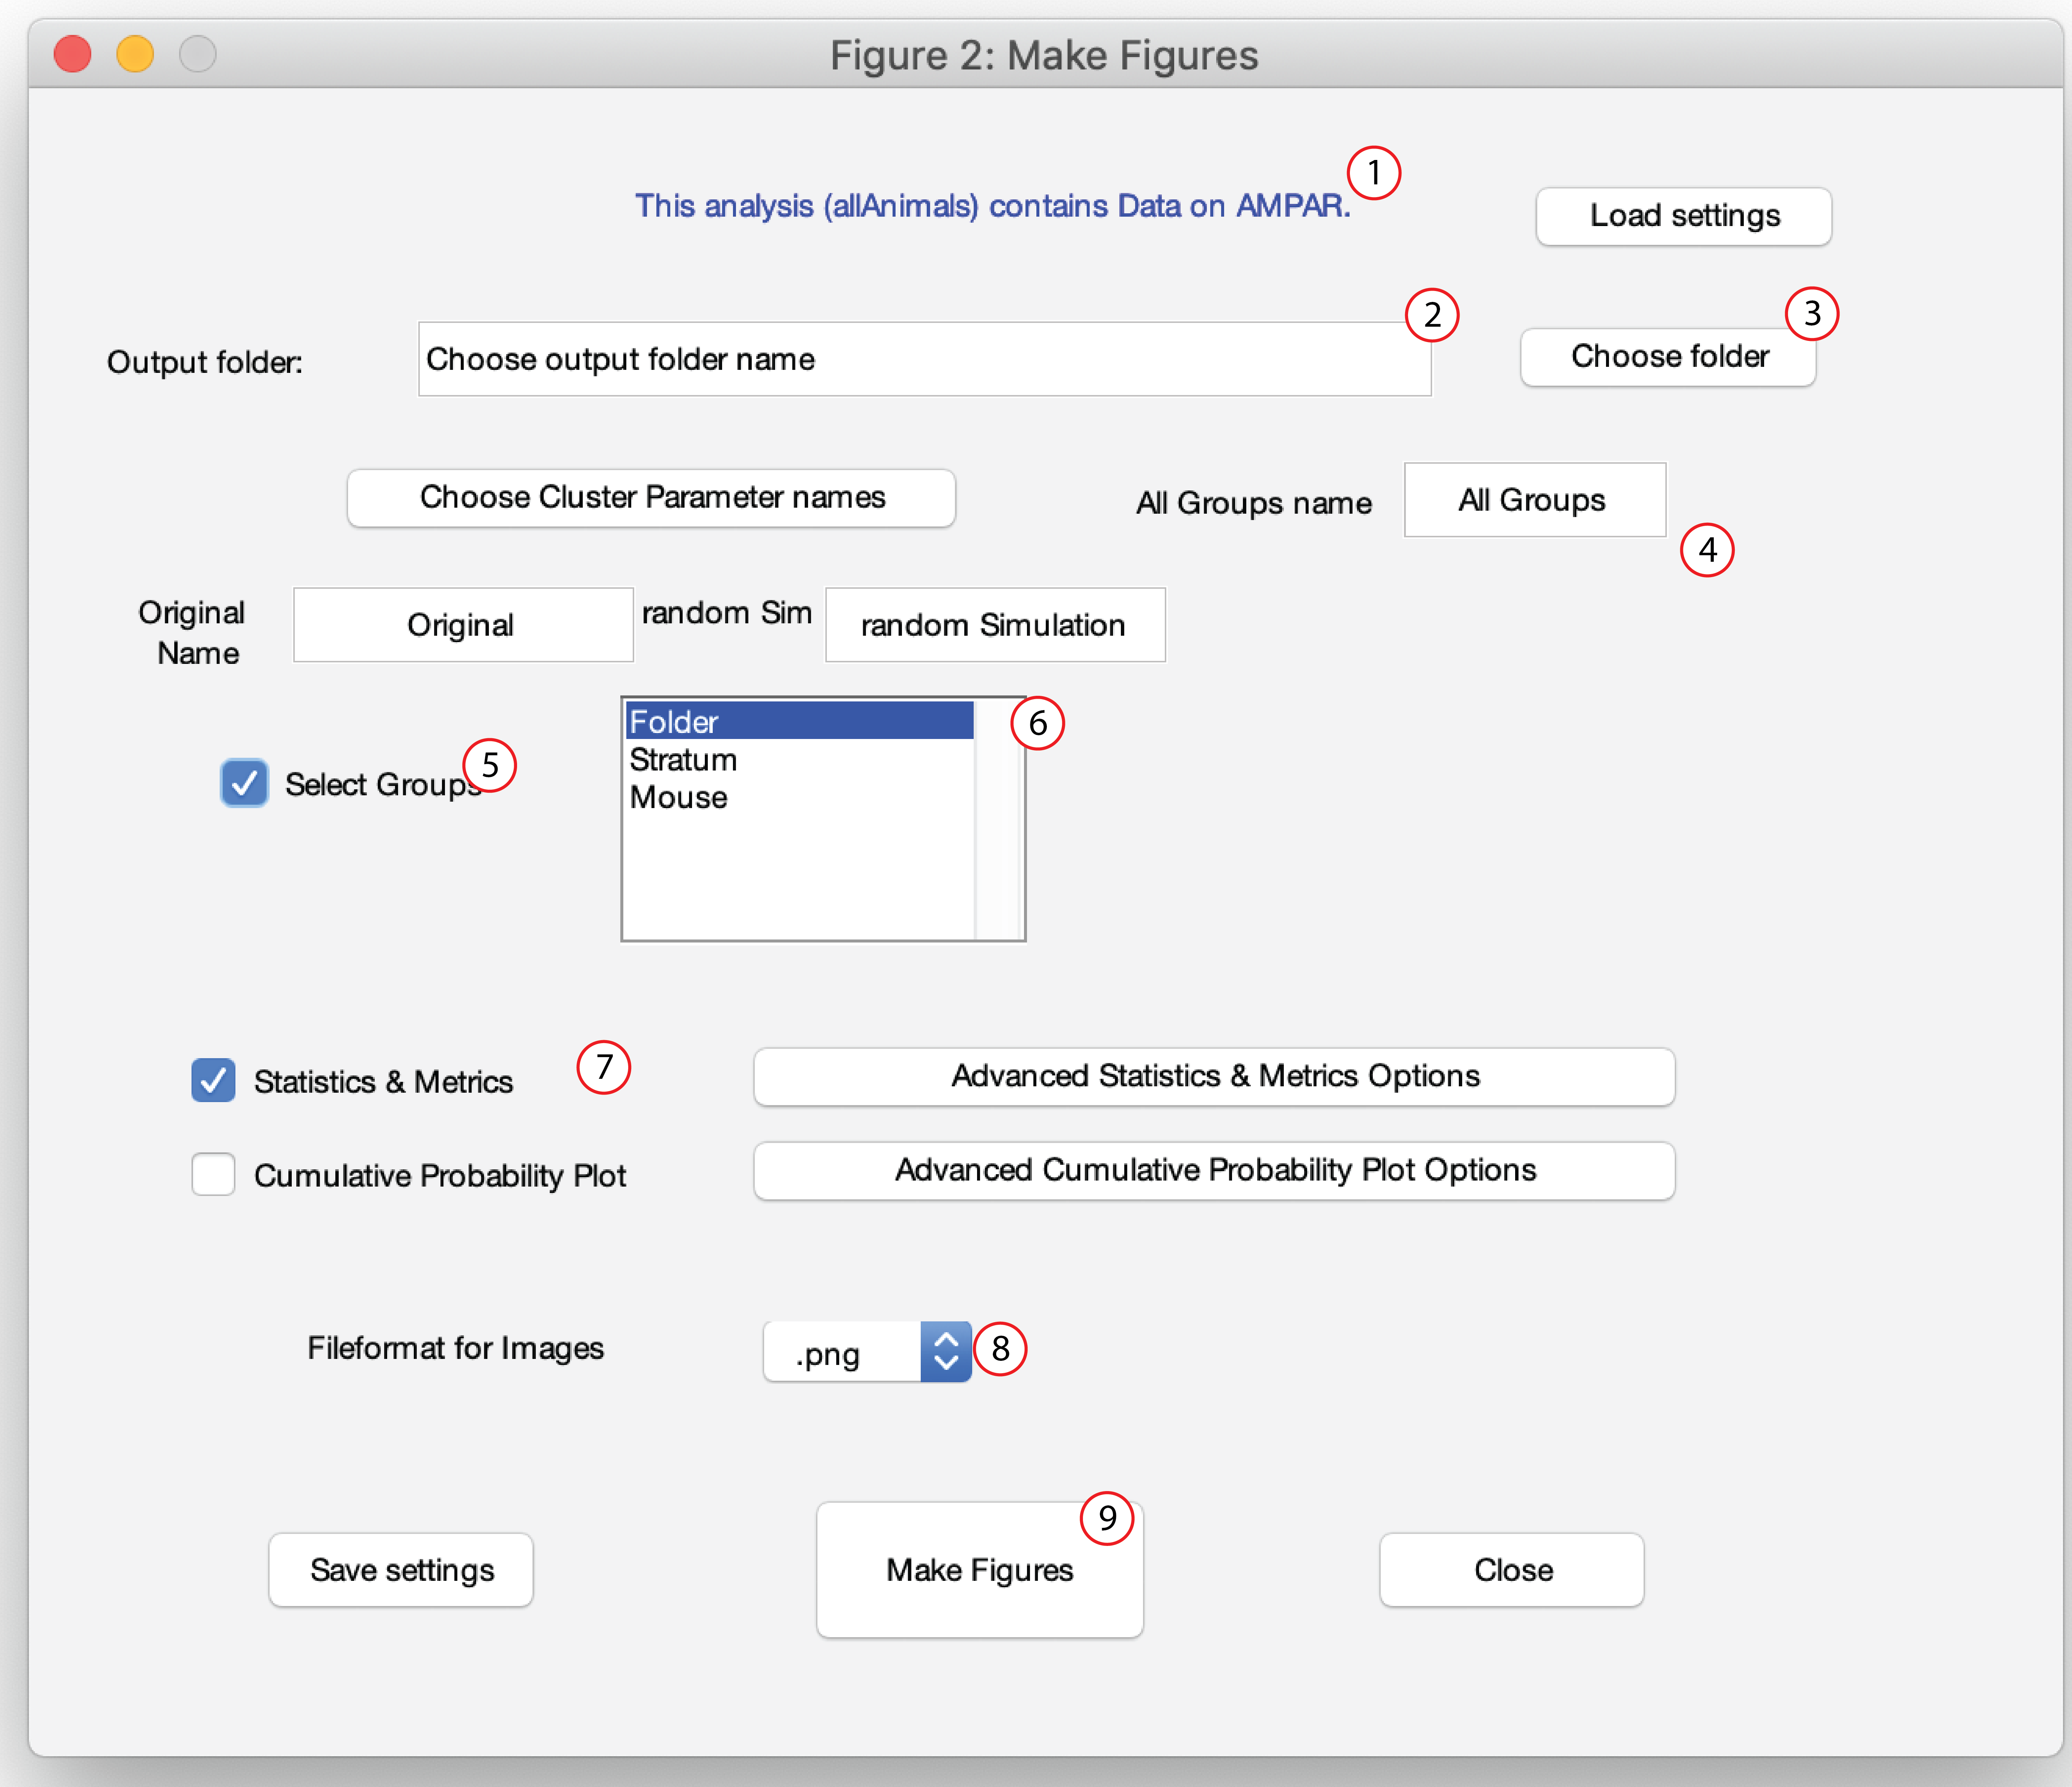
\includegraphics[scale=0.5]{screenshots/scr_Figures.png}
\captionsetup{singlelinecheck=off}
\caption[thing]{Make Figures. 
\begin{enumerate}[label=\textbf{\arabic*:}, leftmargin=1.88\parindent]
\item Shows the name of the analysis and the name of the particles analyzed
\item Path to the selected output folder
\item Select an output folder. As there will be a lot of files generated, we suggest selecting an empty folder.
\item How different things should be named in the resulting datasheets and figures. Right now this naming selection is not followed through in all datasheets and we suggest to largely ignore it. It may be removed or modified in the future.
\item If ticked, you may select based on which groupings the data should be separated. Not ticking is equivalent to selecting all groupings in (6).
\item Select the groupings based on which the data should be divided. In this example, if I select Stratum but not Mouse, data will be seperated based on stratum but individual mice will be pooled.
\item Which kinds of data sheets and figures to create. For a standard analysis we recommend ticking statistics and metrics and not changing advanced options.
\item Which file format generated images should have.
\item Make figures and tables
\end{enumerate}}
\end{figure}
\subsubsection{The Output files}
When making figures, the following directories and files are created in the selected output folder:
\begin{figure}[H]
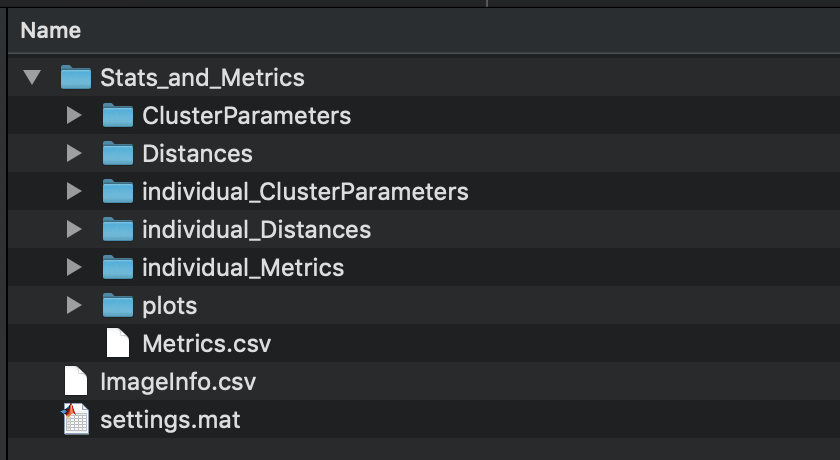
\includegraphics[scale=0.7]{screenshots/scr_output.png}
\captionsetup{singlelinecheck=off}
\caption[thing]{Folderstructure in the output folder}
\end{figure}
ImageInfo.csv contains a list of all images with their scales and the groups they belong to. settings.mat saves the settings used for making these results.

Within the Stats\_and\_Metrics folder there are:\\
Metrics.csv contains descriptive statistics on particle number, demarcated area and particle density for all particle sizes.

The directories "ClusterParameters" and "Distances" contain statistical information about distances and clusterparameters. Files are named <Measured Property>\_<type of statistics>.csv.\\
The <types of statistics> are: "descriptiveStats" - contains mean, standard deviation (STD), standard error (SEM) and median. "analyticStats" - contains pairwise comparisons between each groups. "1by1" - contains an imagewise comparison between real and simulations, it is measured in how many percent of images the measured property is significantly smaller or larger than expected from simulations. "Popmeans" - Tests whether the average of the measured property is different between real and simulation using a paired t-test (pairing is done in an image-wise manner).

The measured properties for ClusterParamaters are: "area" - size of the cluster area. "density" - particle density within the cluster. "excluded Clusters" - number of clusters that were excluded from analysis (Clusters are excluded when all particles are in an exact line, because such clusters have no area. This number should be very close to 0. Large numbers indicate a problem in the analysis). "interDistance\_x" - Distance from clusters of x nm particles to clusters of other particle sizes. "intraDistance" - Distance between clusters of the same particle size. "number" - number of clusters per image. "overlap\_x" - Overlap between cluster areas of clusters of x nm particles and clusters of other particle sizes. "particles" - number of particles per cluster. "thresholdDist" - maximum distance between particles which still counts them as belonging to the same cluster (see \ref{m:clusters} for details).

The measured properties for Distances are: "All\_Distances" - Distances between each pair of particles. "Distance\_from\_Center" - Distance from the center of gravity of the ROI (in nm). "Distance\_from\_Edge" - Distance from the edge of demarcation (in nm). "NND" - Nearest neighbour distance between particles. "normalized\_Distance\_from\_Center" - $ \frac{Distance\_from\_Center}{Distance\_from\_Center + Distance\_from\_Edge} $. 

The directories starting with "individual" contain the unaggregated raw measurements. For individual\_ClusterParameters the files are named <Groupname>\_<SimulationType>.csv. For the real data no simulation type is specified. For individual\_Distances the files are named <Groupname>\_<Distance>.csv. The distances are either of form "Xnm to Ynm" and then contain measurements of distances from Xnm particles to Ynm particles, or of the form "Xnm" and then contain measurements between Xnm particles or from Xnm particles to center or edge. The individual\_Metrics folder contains files name <Groupname>.csv. These contain information of number of particles, ROI area and density of particles for each image.

The directory "plots" contains plots of particle number against ROI area and of particle numbers of different sizes against each other. 
\subsection{Visualizing results}
\label{m:visualize}
This is useful for creating example images.
\begin{figure}[H]
\includegraphics[width=\linewidth]{screenshots/scr_Visualize.png}
\captionsetup{singlelinecheck=off}
\caption[thing]{Visualize Results. Please refer to Fig.\ref{fig:dPoly} for buttons already described there.
\begin{enumerate}[label=\textbf{\arabic*:}, leftmargin=1.88\parindent]
\item When exporting the image, it will look the same as the image shown in this panel
\item Display labels for particles or not
\item Display labels for clusters or not
\item Select simulation from which to show simulated particles
\item Show scalebar or not
\item Displays center of gravity of the demarcation or not
\item Visualization settings, including particle color, how demarcation and outer rim should be displayed. See Fig.\ref{fig:Vis_Options} for details.
\item Hide image and display only labels on a white background
\item When exporting image, additional information (such as zoom size, zoom coordinates, ...) can be saved, so that exact image could be reproduced if minor changes are needed
\item Export image. You may select a path where to save the exported image and specify a fileformat.
\end{enumerate}}
\end{figure}
\begin{figure}[H]
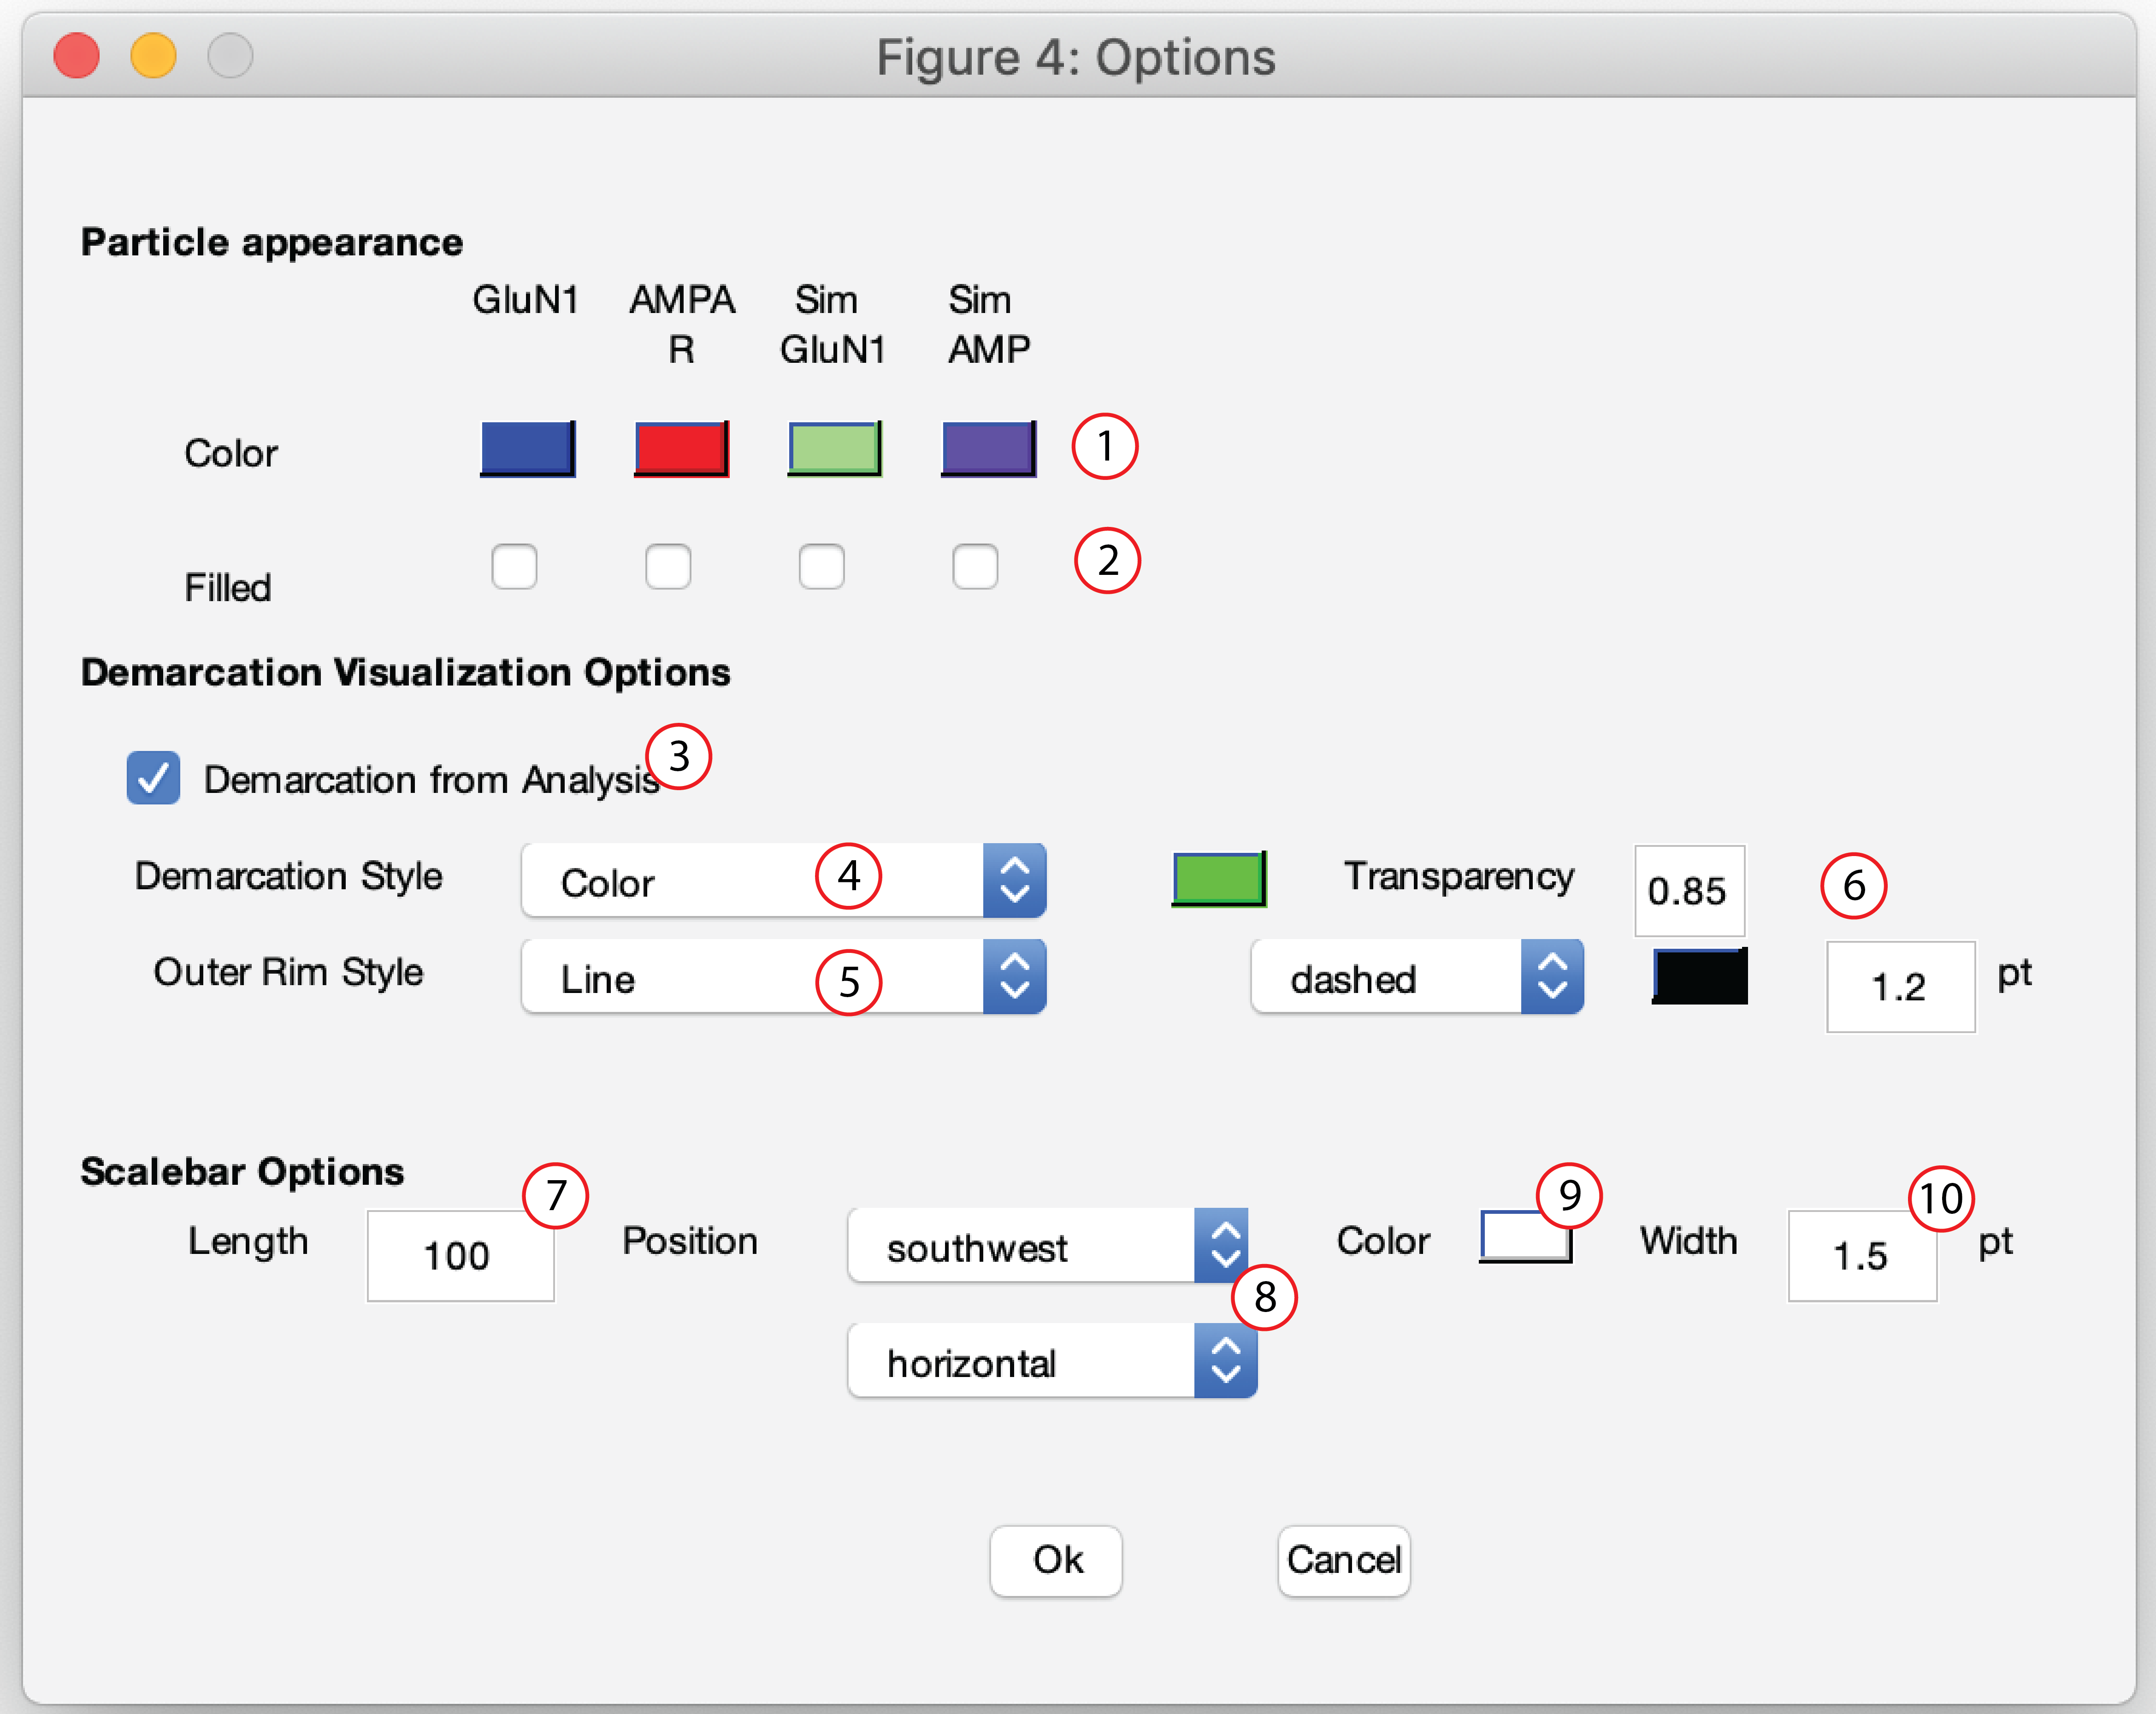
\includegraphics[scale=0.55]{screenshots/scr_VisualizeOptions.png}
\captionsetup{singlelinecheck=off}
\caption[thing]{Visualize Options
\begin{enumerate}[label=\textbf{\arabic*:}, leftmargin=1.88\parindent]
\item Color of real and simulated particle labels
\item Whether the particle label should be filled (filled circle) or not (ring).
\item The demarcation can be either taken from the analysis or from the current demarcation file. If you changed the demarcation after you ran the analysis, different demarcations will be displayed.
\item How to display the demarcation: "None" -> don't display it. "Color" -> Show a color overlay. "Line" -> show a line at the outline. "Brightness" -> Make background darker.
\item Same as (4) but for outer rim
\item Several Options for displaying demarcation and rim style, depending on the style selected in (4) and (5)
\item Length of the scalebar in nm
\item Position of the scalebar within the image
\item Scalebar color
\item Scalebar line thickness
\end{enumerate}}
\label{fig:Vis_Options}
\end{figure}
\section{Training automated analysis}
Training particle detection can be done on CPU. Preparing dataset for demarcation prediction can be done on CPU. Training demarcation prediction should be done on GPU (will take very very long otherwise).
\subsection{Training particle detection}
\label{m:trainPart}
\begin{figure}[H]
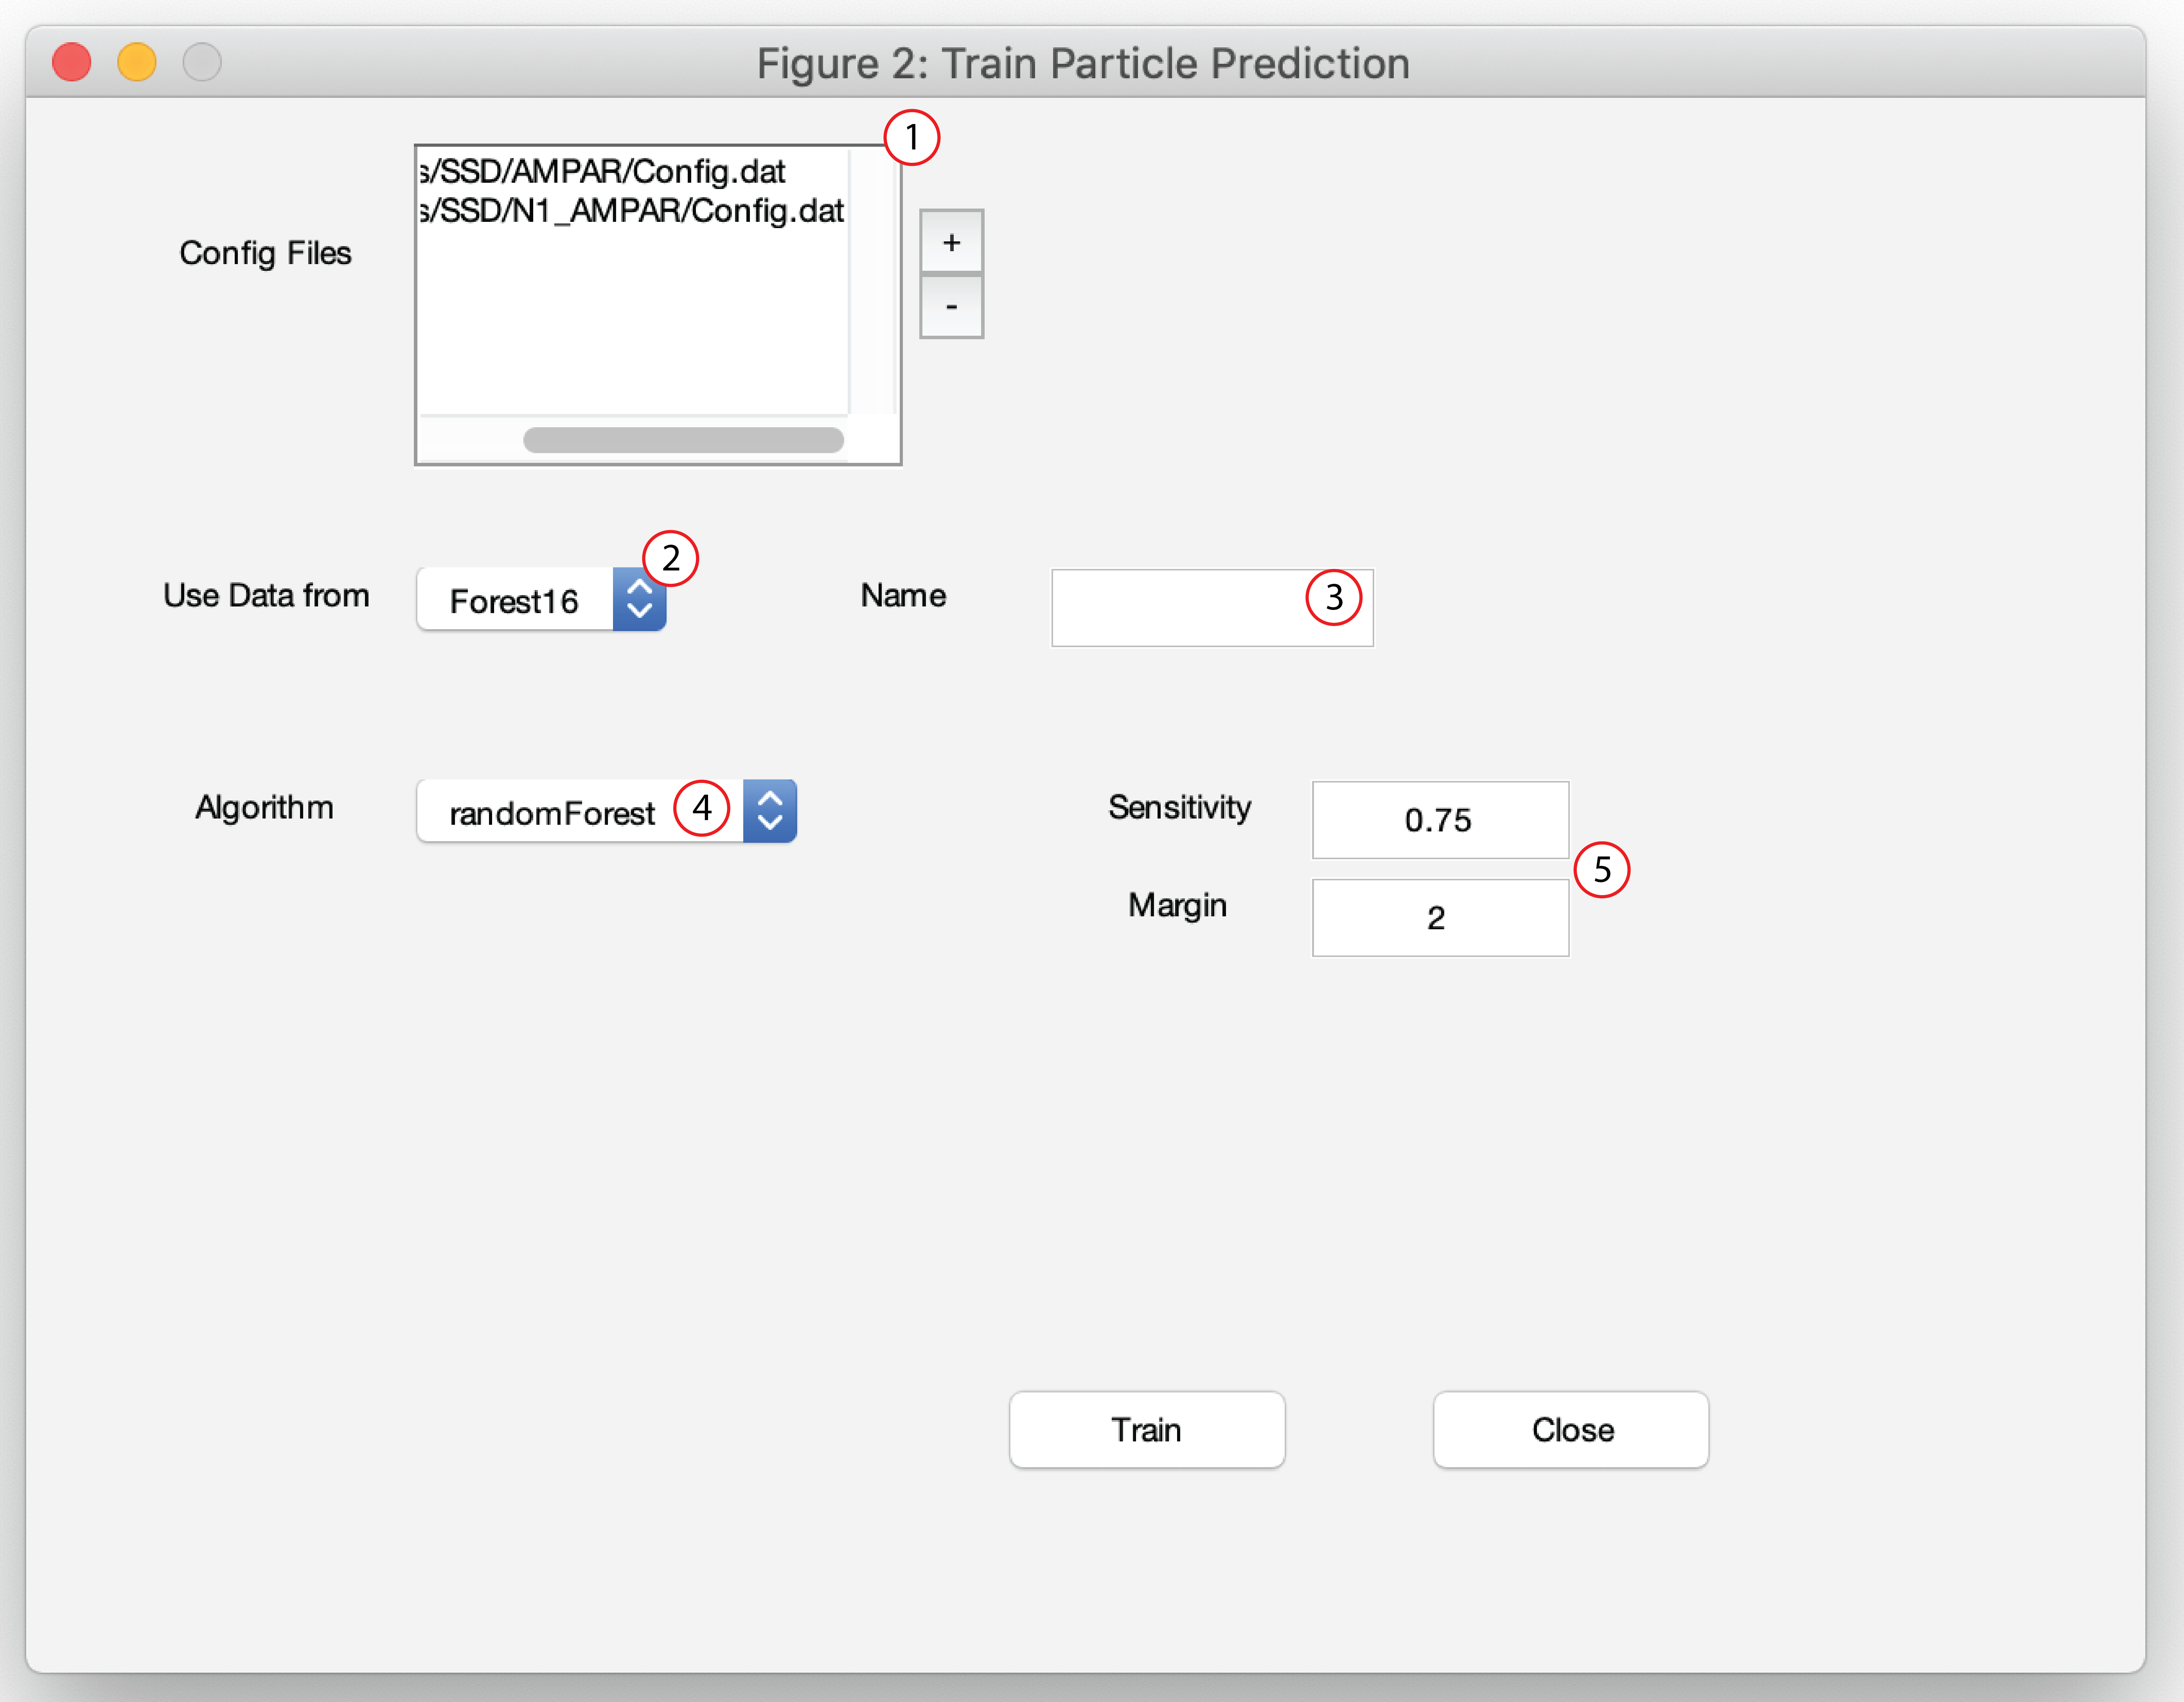
\includegraphics[scale=0.55]{screenshots/scr_ParticleTraining.png}
\captionsetup{singlelinecheck=off}
\caption[thing]{Training particle detection
\begin{enumerate}[label=\textbf{\arabic*:}, leftmargin=1.88\parindent]
\item Select which project files to train on. You may use (+) and (-) buttons to add or remove project files. \emph{Important: Particle anntation in these files has to be completed, otherwise trained classifier will learn the wrong thing}
\item Training data used in already trained classifiers can be reused for training the new one (this is very quick). Select from which classifier trained data should be use or select "None" to train a fresh classifier
\item Name of your new classifier. If you specify one of the names shown in (2), it will overwrite this classifier
\item Which algorithm to use for training your classifier
\item Sensitivity and margin to use for circle detection algorithm. See Fig.\ref{fig:particles} for explanation.

\end{enumerate}}
\end{figure}

\subsection{Training demarcation}
\label{m:trainDem}
For training deep neural networks for automatic demarcation we suggest to create a dataset with the following structure:
\begin{figure}[H]
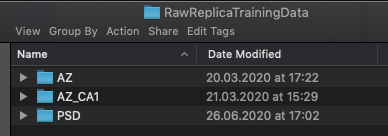
\includegraphics[scale=0.55]{screenshots/scr_dataset.png}
\captionsetup{singlelinecheck=off}
\caption[thing]{Dataset structure}
\end{figure}
Each folder corresponds to a feature (e.g. active zone, PSD) you would like to train. Copy your project (<projectname>.dat and all the folders containing the images) into the folder specifying the appropriate feature. From this folder a dataset with ready to train images can be prepared (see below). \\
If at a later point more fully analyzed projects for the same feature become available, they can simply be copied into the dataset and "prepare dataset" can be rerun. Than the new images will be included for the training. Theoretically, when always adding the latest finished project to the dataset and rerunning training, this should lead to constant improvements of the accuracy of the automated prediction.

\begin{figure}[H]
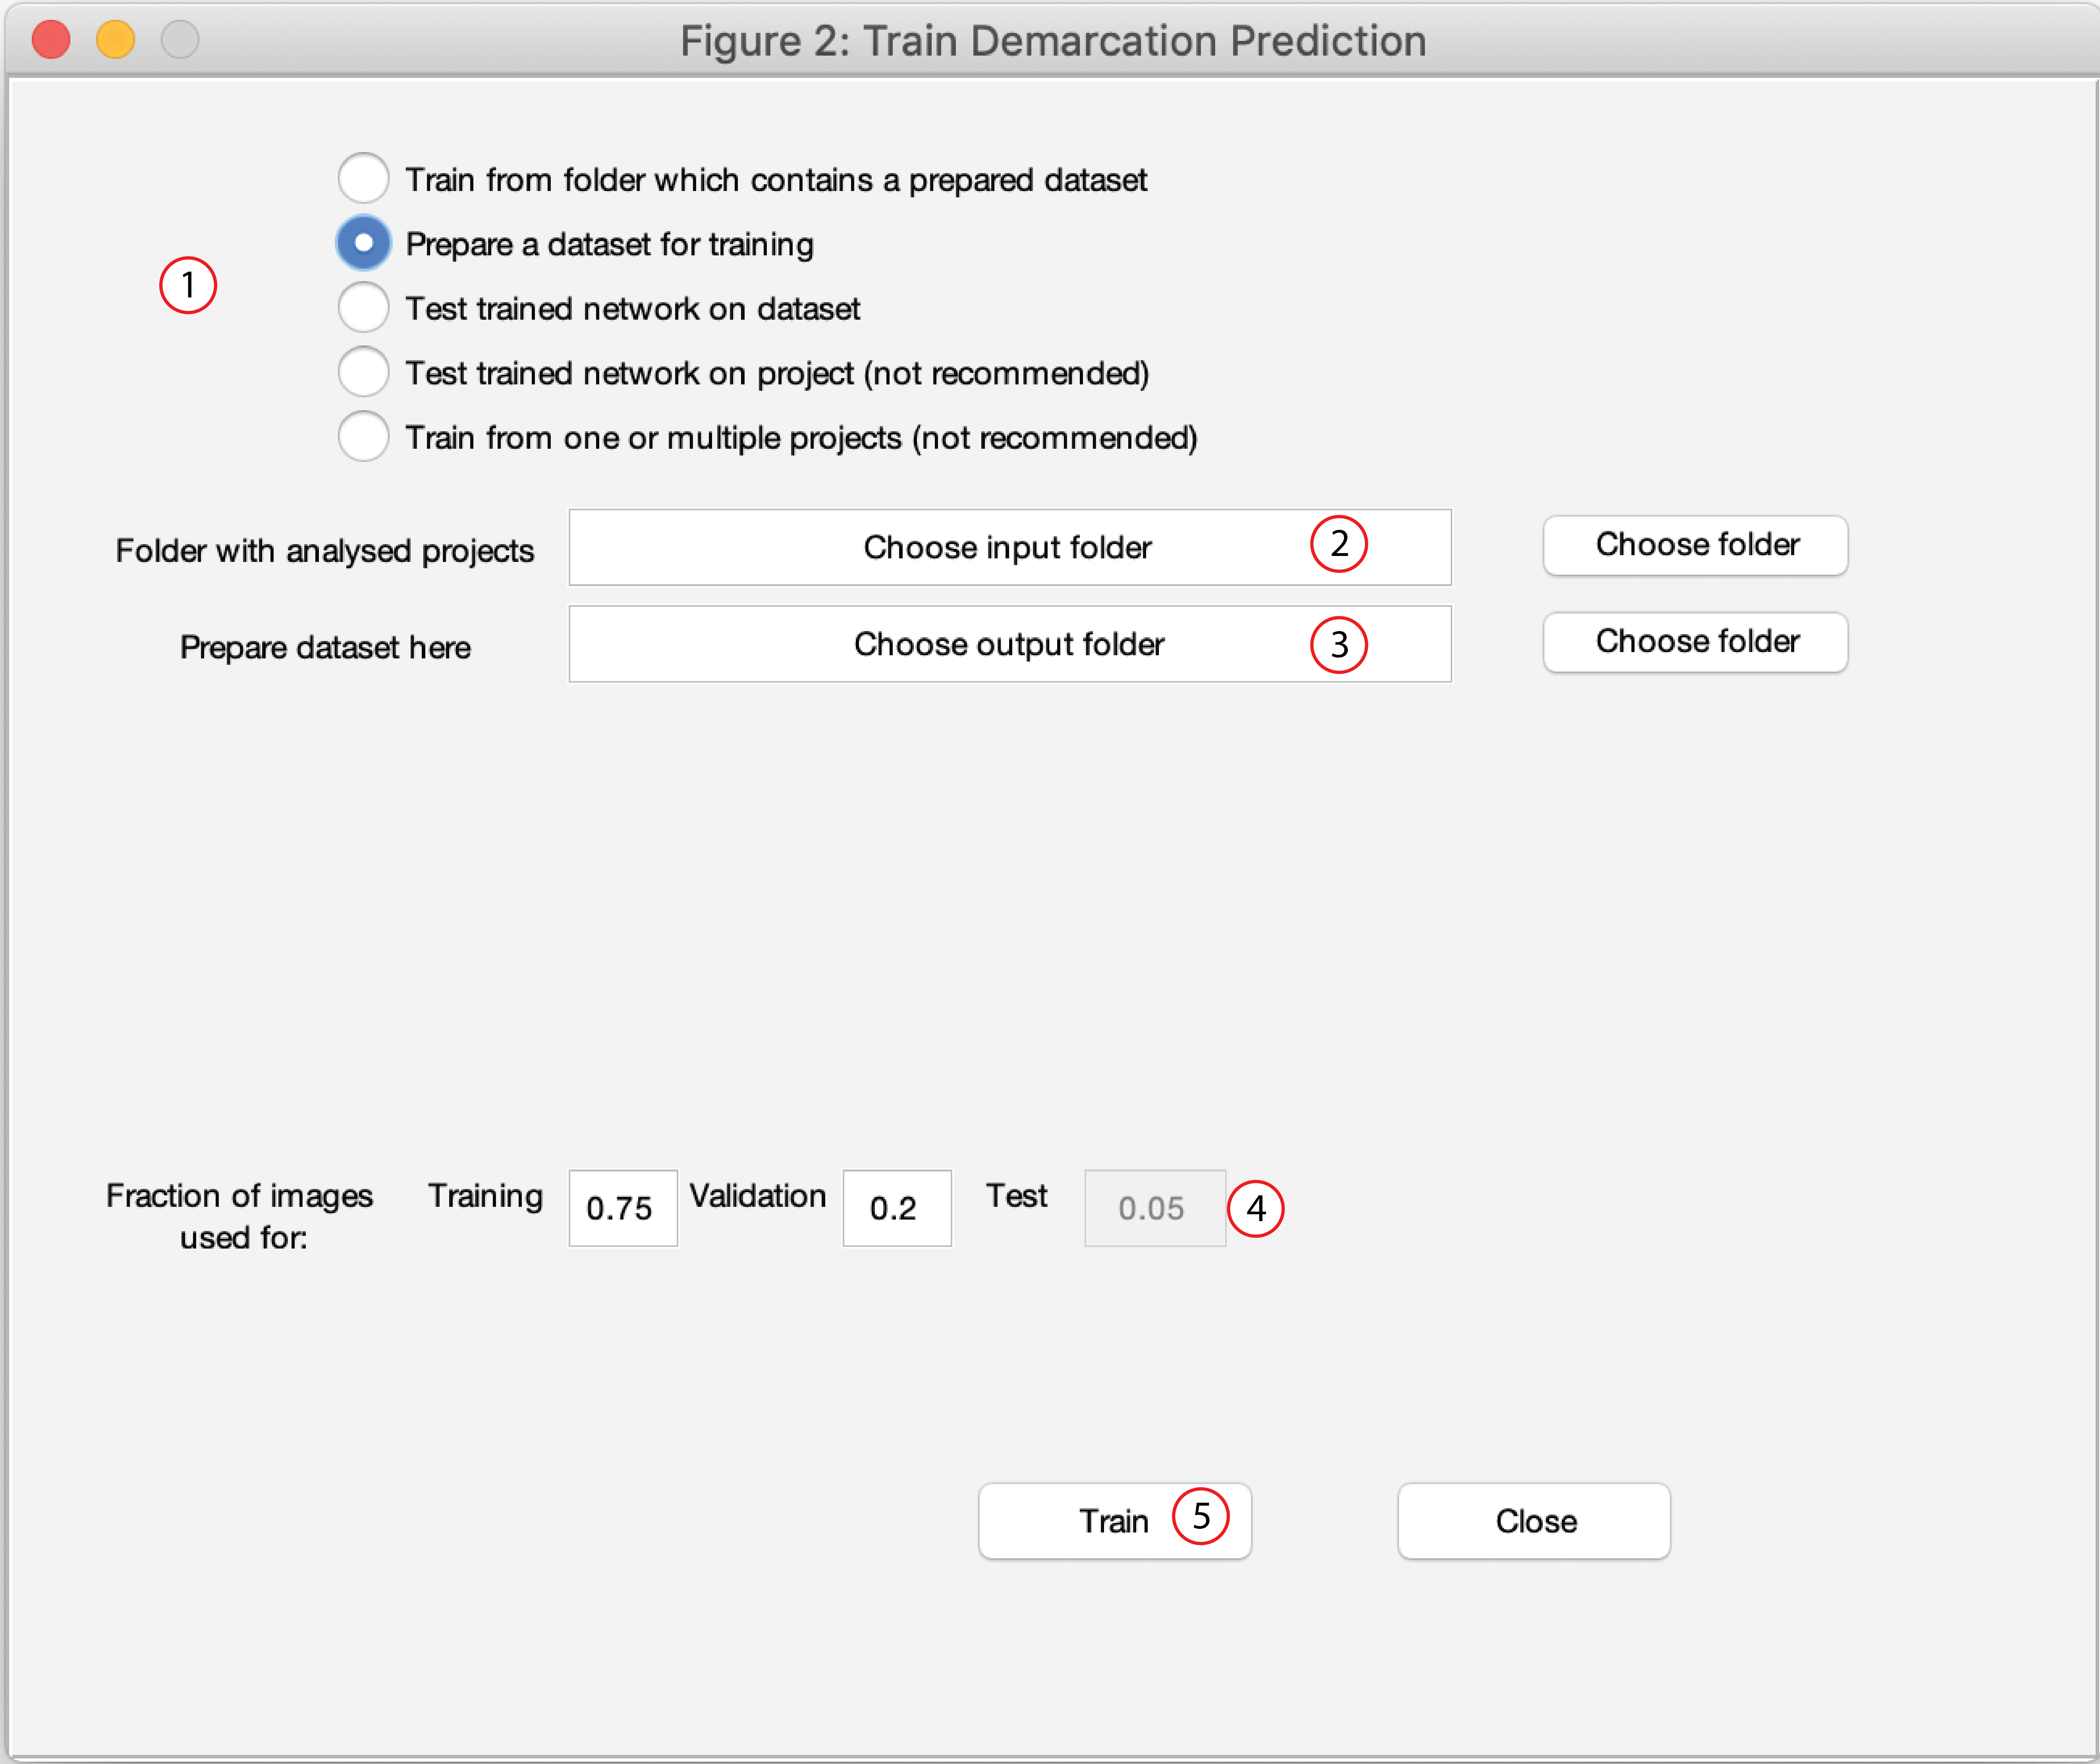
\includegraphics[scale=0.55]{screenshots/scr_TrainDataset.png}
\captionsetup{singlelinecheck=off}
\caption[thing]{Preparing an image dataset for training
\begin{enumerate}[label=\textbf{\arabic*:}, leftmargin=1.88\parindent]
\item Select Prepare dataset
\item Choose the folder with the dataset (see above)
\item Choose the folder which will contain your prepared dataset. (Should be empty or contain a dataset previously prepared from the same folder with annotated projects (more projects could be added since then))
\item Clicking train will now convert your images to make them ready for training. This will take some time.
\item What fraction of images should be used for training, validation and testing (since they need to add up to 1, Test is automatically calculated based on the other two). 
\end{enumerate}}
\label{fig:prepDataset}
\end{figure}

\begin{figure}[H]
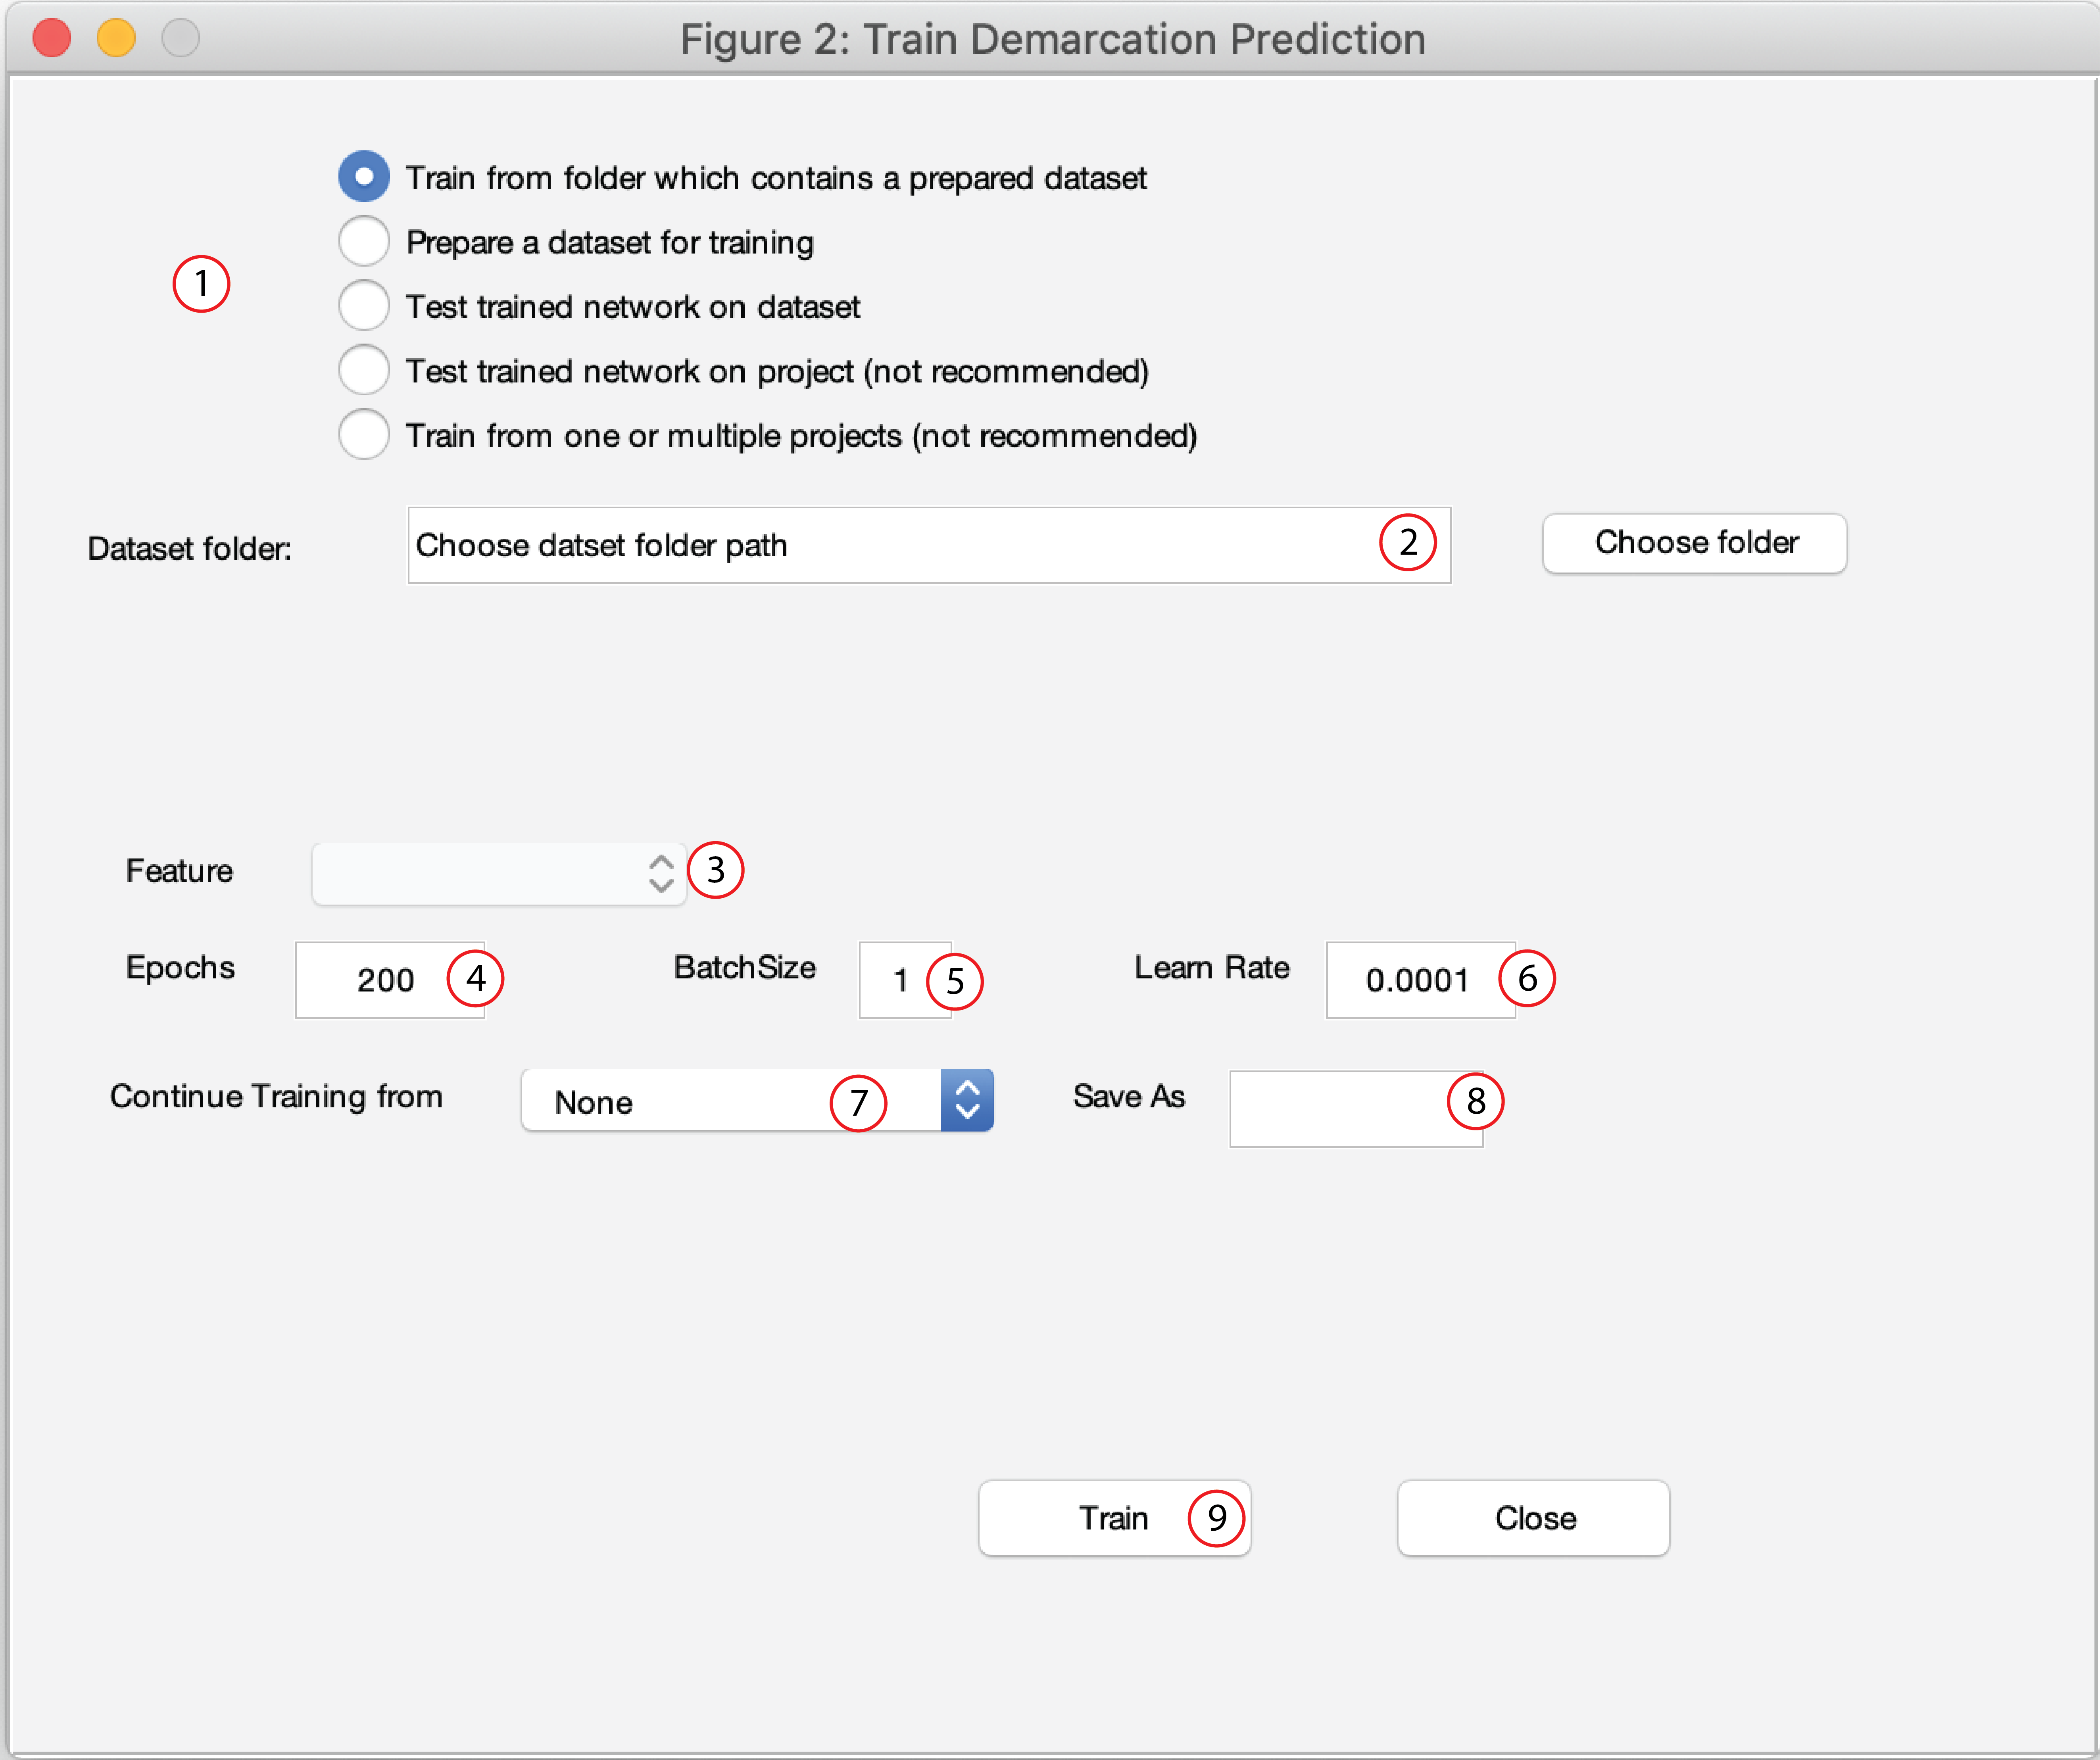
\includegraphics[scale=0.55]{screenshots/scr_DemTraining.png}
\captionsetup{singlelinecheck=off}
\caption[thing]{Train deep neural network for demarcation
\begin{enumerate}[label=\textbf{\arabic*:}, leftmargin=1.88\parindent]
\item Select train from prepared dataset
\item Choose the folder containing your dataset. This is the same folder as specified in (3) at Fig.\ref{fig:prepDataset}.
\item Choose which feature to train from.
\item Number of epochs. During each epoch, the network will be trained on each image of the training dataset once. The higher this number, the longer it takes but the better the result.
\item How many images should be processed at the same time. Unless your GPU has a very large memory, leave unchanged.
\item How fast the network should learn. Higher rates will speed up the learning but may deteriorate performance.
\item Training can be continued from a previously trained network which will result in much fewer needed epochs for reaching a good performance
\item The name under which the newly trained network should be saved. When you specify a name that already exists (see list in (7)), that one will be overwritten.
\item Click train to start training. Depending on number of training images and epochs this may take up to a few days (on GPU) or multiple weeks (CPU).
\end{enumerate}}
\label{fig:trainDem}
\end{figure}

Rather than creating a dataset and training from it, directly training from one or more projects is also possible. Except for quick testing of training parameters, this is not recommended for multiple reasons: 1) Images have to be converted into a dataset anyway, but since it is not saved, this has to happen every time leading to (slightly) increased training times. 2) For the same reason, the training/validation images will change every time (as they are randomly picked to reduce bias). This can lead to performance problems ("Overfitting") when retraining the network multiple times on the same project. 3) Sometimes there is more than one region of interest on an image. Usually these are analysed by duplicating the image and selecting one ROI each. If uncorrected, this will cause problems because the network will see the same image, but has to guess which of the ROI would be appropriate, which will reduce performance When preparing a dataset, but not when training from a project, this issue is corrected for. 

\section{Advanced sections}
\subsection{How Darea stores data and modifying defaults}
\subsubsection{Project files}
Project files (saved as <projectname>.dat) store the relative paths of the images, their primary group (which corresponds to the folder in which they are in) and their scale (in nm/px). They look like this:
\begin{lstlisting}[belowskip=0pt]
GROUP,	ROUTE,	PIXELSIZE
PF_Syn,	PF_Syn/01_37984_F1_II,	0.3
PF_Syn,	PF_Syn/02_37984_F1,	0.3
\end{lstlisting}
Columns are seperated by commas and tabs. Images can be manually added to and removed from a project by modifying this file.
\subsubsection{Project Settings and modifying defaults}
Project settings files (saved as <projectname>\_options.dat) store all settings variable differing from the default.
All default values (including some which cannot be changed in the GUI) are stored in configDefault\_options.dat in the Darea main folder. Here's a small part of it as example:
\begin{lstlisting}[belowskip=0pt,breaklines=true]
#General
particleTypes	[5,10] 	#Particle Diameters
dilate	0	#Size of outer rim in nm
onlyParticlesWithin	true   #Only particles within area of interest should be taken into account

BackgroundBrightness	0.7 	#How much darker the non demarcated area should be

#Analysis
nrsim	50      #Default number of simulations
allName	'All'
SimOptions.mindistance	10
\end{lstlisting}
Setting names and values are separated by tabs and \# can be used for commenting.
Changing these values in this file will modify the default behaviour for all projects. Adding any of these settings to the project settings file will change this for that project only.
For example, writing
\begin{lstlisting}[belowskip=0pt]
nrsim	100
\end{lstlisting}
into the project settings file (create it yourself if it doesn't exist) will cause the default number of simulations in Fig.\ref{fig:analysis} (5) to be 100.

\subsubsection{Groups}
Groups are saved as <projecname>\_groups.dat which look like this:
\begin{lstlisting}[belowskip=0pt]
Image,Folder,Stratum,Mouse
M3-MS5L-A1-AMPAR/001_150000x,M3-MS5L-A1-AMPAR,Radiatum,MS5
M3-MS5L-A1-AMPAR/002_150000x,M3-MS5L-A1-AMPAR,Radiatum,MS5
M3-MS5L-A1-AMPAR/003_150000x,M3-MS5L-A1-AMPAR,Radiatum,MS5
\end{lstlisting}
The first column contains the path to each image, the other columns show the different groupings.
Elements are separated with commas.

\subsubsection{Demarcations}
For each image the demarcation is stored in a <imagename>\_mod.tif file, which is a grayscale image where white denotes background and any other color denotes ROI.
\subsubsection{Particle annotations}
Particle annotations for each image are stored in a <imagename>dots.csv file, which looks like the following:
\begin{lstlisting}[belowskip=0pt]
513.9198, 464.5443, 3.2260, 3.0
625.0329, 500.4324, 3.2260, 3.0
386.2429, 340.1549, 6.4520, 6.0
551.6772, 399.8392, 6.0488, 6.0
\end{lstlisting}
Each row is one particle. The columns are: X and Y coordinates, measured radius and theoretical radius of the particle (all in nm). Elements are separated with commas.
\subsubsection{Analysis results}
Analysis results are stored as <projectname>\_<analysisname>.mat files.
\subsection{Deep learning using the command line}
When wanting to train when no graphical user interface (such as when running it on a cluster) is necessary or possible, only the python/SemanticSegmentationSuite folder is necessary.
Running the training can be done using the following command:
\begin{lstlisting}[belowskip=0pt,breaklines=true]
python <path to SemanticSegmentationSuite>/train.py  --learn_rate "<learn_rate>" --batch_size "<batch_size>" --num_val_images "-1" --num_epochs "<nrEpochs>" --dataset_path "<path to dataset>" --dataset "<feature name>" --save_best "1" --h_flip "1" --v_flip "1" --brightness "0.5" 
\end{lstlisting}
The terms between <> have to be replaced accordingly. <path to dataset> should be the path to the folder where the prepared dataset is located, same as what you would select in Fig.\ref{fig:trainDem} (2). The other terms should be filled the same way as the elements in Fig.\ref{fig:trainDem}. More options are possible, refer to SemanticSegmentationSuite/train.py for details. 
Take care to first install all the appropriate python packages (an environment file we use for our cluster is available as Darea\_LinuxCluster\_GPU.yml) and make sure that the python command links to the proper env having these packages.

\end{document}
